\documentclass[12pt]{extarticle}
\usepackage[T1]{fontenc}
\usepackage{amsmath}
\usepackage{amssymb}
\usepackage[final]{graphicx}
\usepackage{animate}
\usepackage{geometry}
\usepackage{float}
\usepackage{subcaption}
\usepackage{listings}
\usepackage{xcolor}
\usepackage{authblk}
\usepackage{newunicodechar}
\usepackage{booktabs}
\usepackage[backend=biber,style=numeric,sorting=none]{biblatex}
\usepackage{authblk}

\usepackage[colorlinks=true,linkcolor=blue,citecolor=blue,urlcolor=blue]{hyperref}

\geometry{a4paper, portrait, margin=1in}
\emergencystretch=2em
\addbibresource{bibliography.bib}

\newunicodechar{−}{-}

% Python code style for lstlisting
\lstset{
    language=Python,
    basicstyle=\ttfamily\small,
    keywordstyle=\color{blue},
    commentstyle=\color{gray},
    stringstyle=\color{teal},
    numbers=left,
    numberstyle=\tiny\color{gray},
    stepnumber=1,
    numbersep=8pt,
    frame=single,
    breaklines=true,
    breakatwhitespace=false,
    showstringspaces=false,
    tabsize=4,
    captionpos=b
}


% Safe image inclusion: compile even when image files are not present.
\newcommand{\safeincludegraphics}[2][]{%
    \IfFileExists{#2}{%
        \includegraphics[#1]{#2}%
    }{%
        \fbox{%
            \begin{minipage}[c][0.25\textheight][c]{0.8\linewidth}
            \centering
            Missing image file:\\[3pt]
            {\ttfamily\detokenize{#2}}
            \end{minipage}%
        }%
    }%
}

% Safe animation inclusion: compile even when extracted animation frames are not present.
% Args: optional animate options, frame rate, frame prefix, first index, last index.
\newcommand{\safeanimategraphics}[5][]{%
    \IfFileExists{#3#4.png}{%
        \animategraphics[#1]{#2}{#3}{#4}{#5}%
    }{%
        \fbox{%
            \begin{minipage}[c][0.25\textheight][c]{0.8\linewidth}
            \centering
            Missing animation frames:\\[3pt]
            {\ttfamily\detokenize{#3}}
            \end{minipage}%
        }%
    }%
}
\usepackage{array}
\graphicspath{{figures/}{Images/}}

\renewcommand{\listfigurename}{List of plots}
\renewcommand{\listtablename}{List of tables}

\title{\Huge \textbf{\textit{Radio Holography for the Deep Synoptic Array}}}
\date{June--August 2026}
\author[1]{Thach Dang}
\author[1]{Stephen Padin}
\affil[1]{Cahill Center for Astronomy and Astrophysics, California Institute of Technology, Pasadena CA 91125, USA}

\begin{document}

\maketitle
\newpage
\tableofcontents
\clearpage
\listoffigures
\listoftables
\clearpage
\section{1-Dimension Fourier Transform Tests}

\subsection{Top Hat Aperture to Sinc Beam}

Assume a one-dimensional top-hat aperture of width $D$,

\begin{equation}
A(x)=
\begin{cases}
1, & -D/2 \le x \le D/2,\\[4pt]
0, & \text{otherwise},
\end{cases}
\label{eq:top-hat-aperture}
\end{equation}

The far-field electric-field beam as a function of angle $\theta$ is given by the Fourier transform of the aperture illumination:

\begin{equation}
B_E(\theta)=\int_{-D/2}^{D/2} e^{-i2\pi x\sin\theta/\lambda}\,dx.
\label{eq:forward-beam-transform}
\end{equation}

Evaluating Eq.~\eqref{eq:forward-beam-transform} gives the equivalent sinc form

\begin{equation}
B_E(\theta)
=D\frac{\sin\!\left(\pi D\sin\theta/\lambda\right)}{\pi D\sin\theta/\lambda}
\equiv D\,\operatorname{sinc}\!\left(\pi D\sin\theta/\lambda\right),
\label{eq:top-hat-beam}
\end{equation}

\noindent At $\theta = 0$, this expression should be interpreted by its limit, giving $B_E(0)=D$.

\subsection{Inverse Fourier Transforming a Sampled Sinc Beam}

To recover the aperture illumination from the angular beam, we numerically apply an inverse Fourier transform. Starting from

Equation~\eqref{eq:forward-beam-transform} generalizes to an arbitrary aperture illumination $A(x)$.

the inverse transform can be written in terms of the angular coordinate as

\begin{equation}
A(x)=\int B_E(\theta)e^{i2\pi x\sin\theta/\lambda}
\frac{\cos\theta}{\lambda}\,d\theta.
\label{eq:inverse-beam-transform}
\end{equation}

The factor $\cos\theta/\lambda$ appears because the Fourier variable depends on $\sin\theta/\lambda$, so

\begin{equation} d\left(\frac{\sin\theta}{\lambda}\right) = \frac{\cos\theta}{\lambda}  d\theta . \end{equation}

In Python, this inverse transform is implemented numerically using the trapezoidal rule:

\begin{equation} A(x_j) \approx \sum_n B_E(\theta_n)e^{+i2\pi x_j\sin\theta_n/\lambda} \frac{\cos\theta_n}{\lambda} \Delta \theta_n . \end{equation}

\begin{lstlisting}[language=Python]
def inverse_beam_transform(theta_rad, beam, x, wavelength):
    theta_rad = np.asarray(theta_rad, dtype=float)
    beam = np.asarray(beam, dtype=complex)
    x = np.asarray(x, dtype=float)


    order = np.argsort(theta_rad)
    theta_rad = theta_rad[order]
    beam = beam[order]

    phase = np.exp(
    1j
    * 2.0
    * np.pi
    * x[:, None] * np.sin(theta_rad)[None, :]
    / wavelength)

    jacobian = np.cos(theta_rad) / wavelength

    integrand = beam[None, :] * phase * jacobian[None, :]

    aperture = np.trapezoid(
        integrand,
        x=theta_rad,
        axis=1
    )

    return aperture
\end{lstlisting}

Here, \texttt{theta\_rad} contains the sampled angles, \texttt{beam} is the electric-field beam $B_E(\theta)$, and \texttt{x} is the set of aperture-plane positions where the reconstructed aperture $A(x)$ is evaluated. The numerical result is shown in Figs.~\ref{fig:sampled_sinc} and \ref{fig:ifft_top_hat}.
\begin{figure}[h]
    \centering
    \safeincludegraphics[width=0.6\linewidth]{Images/sampled_sinc.png}
    \caption{Sampled Beam Sinc Function}
    \label{fig:sampled_sinc}
\end{figure}
\begin{figure}[h]
    \centering
    \safeincludegraphics[width=0.6\linewidth]{Images/ifft_top_hat.png}
    \caption{Inverse Fourier Transformed the Sampled Beam to get back Top Hat}
    \label{fig:ifft_top_hat}
\end{figure}

\subsection{Implications for Holography}
The aperture field and the measured far-field beam are Fourier transform pairs. This means that the way we sample the beam directly determines what we can recover in the aperture plane. In particular, the number of beam samples determines the total size of the reconstructed aperture plane, while the angular extent of the sampled beam determines the spacing, or gap, between points in the reconstructed aperture.

For the top-hat aperture and its far-field beam, use Eqs.~\eqref{eq:top-hat-aperture} and \eqref{eq:top-hat-beam}.

Based on the optics of single-slit diffraction, the first minima of the sinc function occur when

\begin{equation}
\frac{D\sin\theta}{\lambda} = \pm 1.
\end{equation}

Therefore,

\begin{equation}
\sin\theta_{\rm min} = \pm \frac{\lambda}{D}.
\end{equation}

For small angles, where $\sin\theta \approx \theta$, this becomes

\begin{equation}
\theta_{\rm min} \approx \pm \frac{\lambda}{D}.
\end{equation}

Thus, the beam must be sampled over at least the angular scale

\begin{equation}
-\frac{\lambda}{D}\lesssim\theta\lesssim\frac{\lambda}{D}
\end{equation}

in order to capture the main lobe of the diffraction pattern.

In the reconstructed aperture plane, if the aperture has width $D$ and is represented by $N$ points, then the spacing, or gap, between aperture samples is approximately

\begin{equation}
\Delta x \approx \frac{D}{N}.
\label{eq:aperture-spacing-approx}
\end{equation}

More exactly, if the grid includes both endpoints,

\begin{equation}
x = \mathrm{linspace}\left(-\frac{D}{2}, \frac{D}{2}, N\right),
\end{equation}

then the spacing is

\begin{equation}
\Delta x = \frac{D}{N-1}.
\end{equation}

Therefore, increasing the number of reconstructed aperture points decreases the gap between aperture samples. However, the true resolution of the reconstructed aperture is also limited by the maximum beam angle sampled. A larger angular range in the beam gives access to higher spatial-frequency information and therefore allows finer aperture structure to be recovered.

In summary,

\begin{equation}
\text{More beam samples}
\rightarrow
\text{larger reconstructed aperture plane},
\end{equation}

\begin{equation}
\text{Larger beam angular range}
\rightarrow
\text{smaller aperture-plane spacing},
\end{equation}

and the aperture-plane spacing is given approximately by Eq.~\eqref{eq:aperture-spacing-approx}.

\section{Antenna Control \& Readout}

\subsection{Pointing Offsets Math}

The CBI pointing-offset calculation converts local spherical offsets $(X,Y)$ into changes in azimuth and elevation. Let $O$ be the original pointing center, $T$ be the offset target point, $Z$ be the zenith, and $Q$ be the pole of the local $(X,Y)$ offset coordinate system.

The local offset coordinates are defined such that $+Y$ points from $O$ toward the zenith, while $+X$ points in the direction of increasing azimuth.

\subsubsection{Derivations}
First consider the local right spherical triangle whose side lengths are $X$, $Y$, and $R$. Here $R$ is the great-circle separation between the original pointing direction and the offset target. The side $R$ is opposite the right angle, so the angle between the sides $X$ and $Y$ is

\begin{equation} 90^\circ . \end{equation}

The angle between the side $X$ and the side $R$ is

\begin{equation} 90^\circ - \theta . \end{equation}

Using the spherical cosine formula,

\begin{equation}
\cos a=\cos b\cos c+\sin b\sin c\cos A.
\label{eq:spherical-cosine-law}
\end{equation}

on the side $R$ gives

\begin{align}
\cos R
&= \cos X \cos Y + \sin X \sin Y \cos(90^\circ) \\[4pt]
&= \cos X \cos Y .
\end{align}

Therefore,

\begin{equation}
\boxed{\cos R=\cos X\cos Y}.
\label{eq:local-separation}
\end{equation}

Next use the spherical sine formula,

\begin{equation} \frac{\sin A}{\sin a} = \frac{\sin B}{\sin b} = \frac{\sin C}{\sin c}. \end{equation}

The side $R$ is opposite the right angle, and the side $Y$ is opposite the angle $90^\circ-\theta$. Therefore,

\begin{equation} \frac{\sin(90^\circ-\theta)}{\sin Y} = \frac{\sin(90^\circ)}{\sin R}. \end{equation}

Using

\begin{equation} \sin(90^\circ-\theta)=\cos\theta, \qquad \sin(90^\circ)=1, \end{equation}

we get

\begin{equation} \frac{\cos\theta}{\sin Y} = \frac{1}{\sin R}. \end{equation}

Thus,

\begin{equation}
\boxed{\sin R\cos\theta=\sin Y}.
\label{eq:local-y-component}
\end{equation}

Now use the spherical analogue formula,

\begin{equation}
\sin a\cos B=\cos b\sin c-\sin b\cos c\cos A.
\label{eq:spherical-analogue}
\end{equation}

For the local right spherical triangle, take

\begin{equation} a=R, \qquad B=90^\circ-\theta, \qquad b=Y, \qquad c=X, \qquad A=90^\circ . \end{equation}

Then

\begin{align}
\sin R \cos(90^\circ-\theta)
&= \cos Y \sin X - \sin Y \cos X \cos(90^\circ) \\[4pt]
\sin R \sin\theta
&= \cos Y \sin X .
\end{align}

Therefore,

\begin{equation}
\boxed{\sin R\sin\theta=\cos Y\sin X}.
\label{eq:local-x-component}
\end{equation}

Dividing the two component equations gives

\begin{align}
\tan\theta
&= \frac{\sin R\sin\theta}{\sin R\cos\theta} \\[4pt]
&= \frac{\cos Y\sin X}{\sin Y} \\[4pt]
&= \frac{\sin X}{\tan Y}.
\end{align}

Therefore,

\begin{equation} \boxed{\tan\theta = \frac{\sin X}{\tan Y}}. \end{equation}

Now consider the horizon-coordinate spherical triangle $ZOT$. The sides are

\begin{equation} ZO = 90^\circ - E, \end{equation}

\begin{equation} ZT = 90^\circ - E', \end{equation}

\begin{equation} OT = R. \end{equation}

The angle at $O$ is $\theta$, and the angle at $Z$ is the azimuth change $\Delta A$.

Using the spherical cosine formula on the side $ZT=90^\circ-E'$ gives

\begin{align}
\cos(90^\circ-E')
&= \cos R \cos(90^\circ-E)
+ \sin R \sin(90^\circ-E)\cos\theta \\[4pt]
\sin E'
&= \cos R \sin E + \sin R \cos E \cos\theta .
\end{align}

Therefore,

\begin{equation} \boxed{\sin E' = \cos R \sin E + \sin R \cos E \cos\theta}. \end{equation}

To derive the azimuth-offset equation, first use the sine formula on triangle $ZOT$:

\begin{equation} \frac{\sin\Delta A}{\sin R} = \frac{\sin\theta}{\sin(90^\circ-E')}. \end{equation}

Since

\begin{equation} \sin(90^\circ-E') = \cos E', \end{equation}

we get

\begin{equation} \sin\Delta A = \frac{\sin R\sin\theta}{\cos E'}. \end{equation}

Now use Eq.~\eqref{eq:spherical-analogue}.

For the triangle $ZOT$, take

\begin{equation} A=\theta, \qquad B=\Delta A, \qquad a=90^\circ-E', \qquad b=R, \qquad c=90^\circ-E . \end{equation}

Then

\begin{align}
\sin(90^\circ-E')\cos\Delta A
&= \cos R\sin(90^\circ-E)
- \sin R\cos(90^\circ-E)\cos\theta \\[4pt]
\cos E'\cos\Delta A
&= \cos R\cos E - \sin R\sin E\cos\theta .
\end{align}

Therefore,

\begin{equation} \cos\Delta A = \frac{\cos E\cos R - \sin E\sin R\cos\theta}{\cos E'}. \end{equation}

Now divide $\sin\Delta A$ by $\cos\Delta A$:

\begin{align}
\tan\Delta A
&=
\frac{\dfrac{\sin R\sin\theta}{\cos E'}}
{\dfrac{\cos E\cos R - \sin E\sin R\cos\theta}{\cos E'}} \\[6pt]
&=
\frac{\sin R\sin\theta}
{\cos E\cos R - \sin E\sin R\cos\theta}.
\end{align}

Therefore,

\begin{equation} \boxed{\tan\Delta A = \frac{\sin\theta\sin R}{\cos E\cos R - \sin E\sin R\cos\theta}}. \end{equation}

The complete intermediate pointing solution is given by Eqs.~\eqref{eq:local-separation}, \eqref{eq:local-x-component}, \eqref{eq:local-y-component}, and the boxed equations immediately above.

\subsubsection{Constant-Elevation Case, \texorpdfstring{$E=E'$}{E=E'}}

Now consider the special case where the target point has the same elevation as the original pointing direction:

\begin{equation} E' = E . \end{equation}

This means the telescope moves only in azimuth. The great-circle distance on the sky is still $R$, but the elevation does not change.

The horizon-coordinate triangle $ZOT$ has the same sides defined above. Since $E'=E$,

\begin{equation} ZT = ZO = 90^\circ - E. \end{equation}

The angle at $Z$ is the azimuth offset $\Delta A$.

Using the spherical cosine law, Eq.~\eqref{eq:spherical-cosine-law},

on the side $OT=R$ gives

\begin{align}
\cos R
&=
\cos(90^\circ-E)\cos(90^\circ-E)
+
\sin(90^\circ-E)\sin(90^\circ-E)\cos\Delta A .
\end{align}

Using

\begin{equation} \cos(90^\circ-E)=\sin E, \end{equation}

and

\begin{equation} \sin(90^\circ-E)=\cos E, \end{equation}

we get

\begin{equation}
\cos R=\sin^2 E+\cos^2 E\cos\Delta A.
\end{equation}

Now solve for $\cos\Delta A$:

\begin{align}
\cos R - \sin^2 E
&=
\cos^2 E \cos\Delta A ,
\end{align}

so

\begin{equation}
\cos\Delta A = \frac{\cos R-\sin^2 E}{\cos^2 E}.
\end{equation}

Using the identity

\begin{equation} \sin^2 E = 1 - \cos^2 E, \end{equation}

we can rewrite the numerator as

\begin{align}
\cos R - \sin^2 E=
\cos R - (1-\cos^2 E) =
\cos R - 1 + \cos^2 E .
\end{align}

Therefore,

\begin{align}
\cos\Delta A=
\frac{\cos R - 1 + \cos^2 E}{\cos^2 E} =
\frac{\cos^2 E}{\cos^2 E}
+
\frac{\cos R - 1}{\cos^2 E}.
\end{align}

Thus,

\begin{equation}
\boxed{
\cos\Delta A
=1+
\frac{\cos R-1}{\cos^2 E}}
\label{eq:simplified-xel-to-az}
\end{equation}

Solving for $\Delta A$ gives

\begin{equation}
\boxed{
\Delta A=\cos^{-1}
\left[
1+
\frac{\cos R-1}{\cos^2 E}
\right]
}
\label{eq:simplified-xel-to-az-solved}
\end{equation}

In the notation of the \texttt{sky\_to\_az} function,

\begin{equation} R = \texttt{sky\_angle}, \end{equation}

\begin{equation} E = \texttt{el}, \end{equation}

and

\begin{equation} \Delta A = \texttt{az\_angle}. \end{equation}

Therefore,

\begin{equation}
\boxed{
\cos(\texttt{az\_angle})=
1+
\frac{\cos(\texttt{sky\_angle})-1}{\cos^2(\texttt{el})}
}.
\end{equation}

This is the exact spherical-trigonometry expression for the azimuth offset required to move a great-circle distance $R$ at fixed elevation $E$.

For small angular offsets, we can approximate

\begin{equation} \cos R \approx 1 - \frac{R^2}{2}, \end{equation}

and

\begin{equation} \cos\Delta A \approx 1 - \frac{(\Delta A)^2}{2}. \end{equation}

Substituting into

\begin{equation}
\cos\Delta A=1+
\frac{\cos R-1}{\cos^2 E},
\end{equation}

gives

\begin{align}
1-\frac{(\Delta A)^2}{2}
&\approx
1+
\frac{
\left(1-\dfrac{R^2}{2}\right)-1
}{
\cos^2 E
}=
1-\frac{R^2}{2\cos^2 E}.
\end{align}

Therefore,

\begin{equation}
\frac{(\Delta A)^2}{2}
\approx
\frac{R^2}{2\cos^2 E},
\end{equation}

so

\begin{equation}
\boxed{
\Delta A \approx \frac{R}{\cos E}
}.
\end{equation}

Thus, for small offsets, the required azimuth motion is larger than the true sky motion by a factor of approximately $1/\cos E$.
\subsubsection{Eliminating \texorpdfstring{$R$ and $\theta$}{R and theta}}

We now eliminate $R$ and $\theta$ so that the final equations are written directly in terms of $X$, $Y$, and the original elevation $E$.

From the local triangle $QOT$, use Eqs.~\eqref{eq:local-separation}, \eqref{eq:local-x-component}, and \eqref{eq:local-y-component}.

Start with the elevation equation,

\begin{equation} \sin E' = \cos R\sin E + \sin R\cos E\cos\theta. \end{equation}

Substitute Eqs.~\eqref{eq:local-separation} and \eqref{eq:local-y-component}.

Then

\begin{align}
\sin E'
&= \sin E\cos Y\cos X + \cos E\sin Y .
\end{align}

Therefore,

\begin{equation} \boxed{E' = \sin^{-1}\left(\sin E\cos Y\cos X + \cos E\sin Y\right)}. \end{equation}

The elevation offset is

\begin{equation} \Delta E = E' - E. \end{equation}

Thus,

\begin{equation} \boxed{\Delta E = \sin^{-1}\left(\sin E\cos Y\cos X + \cos E\sin Y\right) - E}. \end{equation}

Next start with the azimuth-offset equation,

\begin{equation} \tan\Delta A = \frac{\sin R\sin\theta}{\cos E\cos R - \sin E\sin R\cos\theta}. \end{equation}

Substitute Eqs.~\eqref{eq:local-x-component}--\eqref{eq:local-separation}.

Then

\begin{align}
\tan\Delta A
&=
\frac{\cos Y\sin X}
{\cos E\cos Y\cos X - \sin E\sin Y}.
\end{align}

Therefore,

\begin{equation} \boxed{\tan\Delta A = \frac{\cos Y\sin X}{\cos E\cos Y\cos X - \sin E\sin Y}}. \end{equation}


Thus, the final equations after eliminating $R$ and $\theta$ are

\begin{equation}
\boxed{
\Delta E = \sin^{-1}\left(\sin E\cos Y\cos X + \cos E\sin Y\right) - E
}
\label{eq:full-pointing-delta-el}
\end{equation}

and

\begin{equation}
\boxed{
\Delta A = \tan^{-1}\left(
\frac{\cos{Y}\sin{X}}{\cos{E}\cos{Y}\cos{X}-\sin{E}\sin{Y}}
\right)
}
\label{eq:full-pointing-delta-az}
\end{equation}
\subsubsection{Do We Need to Use the Full Equation?}

The simplified azimuth correction, Eq.~\eqref{eq:simplified-xel-to-az},

is useful for estimating how a sky angle maps into an azimuth angle at a given elevation. However, this approximation does not fully account for the coupled geometry between azimuth, elevation, and the two-dimensional sky offsets. In particular, when the beam is offset in both the $X$ and $Y$ directions, the true azimuth and elevation offsets are coupled through the pointing geometry.

The full elevation and azimuth offsets are Eqs.~\eqref{eq:full-pointing-delta-el} and \eqref{eq:full-pointing-delta-az}.

The comparison between the real offset equations and the simplified \texttt{sky\_to\_az} approximation shows when the simplified relation is valid and when it begins to fail. At low elevation, especially at $E=0^\circ$, the two methods should match exactly. This is because the projection geometry becomes simple: azimuthal motion maps directly onto the sky $X$ direction, and elevation motion maps directly onto the sky $Y$ direction. Therefore, at $E=0^\circ$, we expect

\begin{equation}
\Delta A_{\rm real}
=
\Delta A_{\rm sky\_to\_az},
\end{equation}

and

\begin{equation}
\Delta E_{\rm real}
=
\Delta E_{\rm sky\_to\_az}.
\end{equation}

This behavior is shown in Fig.~\ref{fig:offsets_from_2_equations}. At $E=0^\circ$, the real offset and \texttt{sky\_to\_az} curves lie on top of each other for both $\Delta A$ and $\Delta E$. In this limit, the simplified equation is sufficient.

\begin{figure}[H]
    \centering
\safeincludegraphics[width = 0.9\linewidth]{Images/offsets_from_2_equations.png}
    \caption{Comparison between the full real offset equations and the simplified \texttt{sky\_to\_az} approximation. At $E=0^\circ$, the two methods agree exactly. As elevation increases, the azimuth offset begins to deviate significantly, especially near $E=90^\circ$.}
    \label{fig:offsets_from_2_equations}
\end{figure}

However, as elevation increases, the azimuth correction becomes increasingly nonlinear. At $E=45^\circ$, the difference between the real azimuth offset and the \texttt{sky\_to\_az} approximation is already visible. By $E=70^\circ$, the real azimuth offset differs substantially from the simplified prediction. Near $E=90^\circ$, the azimuth coordinate becomes nearly singular, so small changes in sky position can correspond to very large changes in azimuth. This causes the largest disagreement between the full equation and the simplified approximation.

The elevation offset behaves differently. For most elevations, the real $\Delta E$ and the \texttt{sky\_to\_az} approximation remain much closer than the azimuth offsets. This means the main geometric failure of the simplified approximation is in the azimuth direction, especially at high elevation.

To test how these differences affect holography, the difference between the real offsets and the \texttt{sky\_to\_az} approximation was added directly to the beam angle. For the azimuth case, the shifted beam is

\begin{equation}
B_{\rm shifted}(\theta)
=
B_E(\theta + \Delta A_{\rm diff}),
\end{equation}

where

\begin{equation}
\Delta A_{\rm diff}
=
\Delta A_{\rm real}
-
\Delta A_{\rm sky\_to\_az}.
\end{equation}

Similarly, for elevation,

\begin{equation}
B_{\rm shifted}(\theta)
=
B_E(\theta + \Delta E_{\rm diff}),
\end{equation}

where

\begin{equation}
\Delta E_{\rm diff}
=
\Delta E_{\rm real}
-
\Delta E_{\rm sky\_to\_az}.
\end{equation}

Figure~\ref{fig:offset_beam_test} shows the resulting shifted beams. If the offsets are not accounted for, the sampled beam no longer follows the ideal top-hat Fourier transform exactly. Some elevations produce only small changes, while others introduce larger deviations in the beam samples. These deviations are especially important because holography uses these sampled beam values to reconstruct the aperture.

\begin{figure}[H]
    \centering
    \safeincludegraphics[width=1\linewidth]{Images/offset_beam_test.png}
    \caption{Effect of adding the azimuth offset differences to the ideal beam. The shifted beam is evaluated as $B_E(\theta+\Delta A_{\rm diff})$, where $\Delta A_{\rm diff}$ is the difference between the full real offset and the simplified \texttt{sky\_to\_az} approximation.}
    \label{fig:offset_beam_test}
\end{figure}

The reconstructed aperture shows the consequence more clearly. If the offsets are not accounted for, the recovered aperture is no longer a clean top-hat. Instead, the aperture reconstruction develops oscillations and amplitude errors. This is shown in Fig.~\ref{fig:offset_aperture_test}. Therefore, even small angular errors in the beam samples can create artificial structure in the aperture plane after the inverse Fourier transform.

\begin{figure}[H]
    \centering
    \safeincludegraphics[width=\linewidth]{Images/offset_aperture_test.png}
    \caption{Reconstructed aperture after applying the offset-shifted beam samples. The ideal reconstruction should recover a top-hat aperture, but uncorrected pointing offsets introduce oscillations and amplitude errors in the reconstructed aperture.}
    \label{fig:offset_aperture_test}
\end{figure}

Therefore, the simplified equation is acceptable at $E=0^\circ$, where the two methods match exactly, but it is not reliable at high elevations. For holography, the full pointing equations should be used because aperture reconstruction is sensitive to small errors in the measured beam positions.

\subsection{Antenna Control Software}
The MNC Client is the recommended Python interface for queue-based antenna control. Direct low-level antenna commands such as parking, stopping, activating, or moving a single antenna are handled by \texttt{antenna-cli}; the MNC Client instead schedules and monitors observations through the MNC server.

\subsubsection{MNC Client}
The MNC Client is a Python interface for communicating with the DSA-2000 Monitor and Control (MNC) server over gRPC. It does not command the antennas directly over MQTT. Instead, it sends requests to the MNC server, which manages the observation queue and, when appropriate, commands the antenna array through the MNC control system.

Before using the Python client from a local machine, an SSH tunnel to OVRO must be open. The SSH configuration should include a local forward for the MNC gRPC port:

\begin{lstlisting}
Host ovro
    User spadin
    HostName ssh.ovro.caltech.edu
    LocalForward 50051 mvp03mncopl.ovro.pvt:50051
\end{lstlisting}

Then start the tunnel from a terminal on the local machine:

\begin{lstlisting}
    ssh ovro
\end{lstlisting}

Keep this terminal open. In a second local terminal, go to the repository and start Python:

\begin{lstlisting}
cd /Users/thachdang/dsa-2000-monorepo
python
\end{lstlisting}

The MNC Client can then connect to the forwarded MNC server using \texttt{localhost} and port \texttt{50051}:

\begin{lstlisting}
from mnc_client import MNCClient

client = MNCClient(host="localhost", port=50051)
client.connect()
\end{lstlisting}

The controller mode can be checked with:

\begin{lstlisting}
from dsa_proto import mnc_pb2
from mnc_client import MNCClient

with MNCClient(host="localhost", port=50051) as client:
    state = client.get_controller_state()
    print(mnc_pb2.ControllerMode.Name(state.mode))
\end{lstlisting}

The MNC controller has three main modes:

\begin{itemize}
    \item \texttt{STANDBY}: safe idle mode. MNC will not start new observations or drive the array.
    \item \texttt{SCIENCE}: normal autonomous observing mode. The observing pipeline may add observations automatically.
    \item \texttt{ENGINEERING}: manual/operator mode. MNC still processes queued observations, but the automated observing pipeline should not add new ones.
\end{itemize}

To set the controller mode:

\begin{lstlisting}
with MNCClient(host="localhost", port=50051) as client:
    client.set_standby()
    # or:
    client.set_science()
    # or:
    client.set_engineering()
\end{lstlisting}

An observation can be added by creating an \texttt{AddObservationRequest}. The observation specifies a source name, RA and Dec in degrees, an allowed start-time window, and a duration. For example, the following schedules a five-minute observation of Cas A that may start between 2 and 30 minutes from now:

\begin{lstlisting}
from datetime import datetime, timedelta, timezone
from google.protobuf.duration_pb2 import Duration
from google.protobuf.timestamp_pb2 import Timestamp
from dsa_proto import mnc_pb2
from mnc_client import MNCClient

now = datetime.now(timezone.utc)

earliest = Timestamp()
earliest.FromDatetime(now + timedelta(minutes=2))

latest = Timestamp()
latest.FromDatetime(now + timedelta(minutes=30))

duration = Duration(seconds=300)

with MNCClient(host="localhost", port=50051) as client:
    resp = client.add_observation(
        mnc_pb2.AddObservationRequest(
            source_name="CasA",
            ra_degrees=350.86,
            dec_degrees=58.81,
            earliest_start_time=earliest,
            latest_start_time=latest,
            duration=duration,
        )
    )

    print("Added observation ID:", resp.id)
\end{lstlisting}

If the controller is in \texttt{SCIENCE} or \texttt{ENGINEERING} mode, MNC will process the queued observation. When the observation reaches its preparation time, MNC converts the RA/Dec target into antenna tracking commands and sends them to the configured antennas.

Queued observations can be checked with \texttt{find\_observations}. To print all currently scheduled observations:

\begin{lstlisting}
from dsa_proto import mnc_pb2
from mnc_client import MNCClient

with MNCClient(host="localhost", port=50051) as client:
    resp = client.find_observations(
        mnc_pb2.FindObservationsRequest(
            status=mnc_pb2.ObservationStatus.SCHEDULED
        )
    )

    for obs in resp.observations:
        print(
            obs.id,
            obs.source_name,
            obs.ra_degrees,
            obs.dec_degrees,
            obs.earliest_start_time.ToDatetime(),
            obs.duration.seconds,
        )
\end{lstlisting}

To print all observations, regardless of status:

\begin{lstlisting}
with MNCClient(host="localhost", port=50051) as client:
    resp = client.find_observations(
        mnc_pb2.FindObservationsRequest()
    )

    for obs in resp.observations:
        print(
            obs.id,
            mnc_pb2.ObservationStatus.Name(obs.status),
            obs.source_name,
            obs.ra_degrees,
            obs.dec_degrees,
            obs.earliest_start_time.ToDatetime(),
            obs.duration.seconds,
        )
\end{lstlisting}

The currently observing observation, if any, can be queried with:

\begin{lstlisting}
with MNCClient(host="localhost", port=50051) as client:
    obs = client.get_observing()

    if obs is None:
        print("No observation is currently active.")
    else:
        print(obs.id, obs.source_name)
\end{lstlisting}
\subsubsection{Low-Level Antenna Control with \texttt{antenna-cli}}

Low-level antenna control is done from \texttt{mvp03}, the MNC infrastructure
server. The normal workflow for custom/manual antenna work is:

\begin{enumerate}
    \item Connect to Tailscale.
    \item Put MNC into \textbf{Standby} mode from the MNC web UI.
    \item SSH into \texttt{mvp03}.
    \item Run \texttt{antenna-cli} commands from the monorepo checkout.
    \item When finished, return MNC to \textbf{Science} mode from the web UI.
\end{enumerate}

Example connection:

\begin{lstlisting}
ssh ntdang@mvp03mncopl.ovro.dsa.pvt
cd /home/ntdang/dsa-2000-monorepo
\end{lstlisting}

The CLI can be run directly with Nix:

\begin{lstlisting}
nix run .#antenna-cli -- --help
\end{lstlisting}

Or it can be built once:

\begin{lstlisting}
nix build .#antenna-cli
./result/bin/antenna-cli --help
\end{lstlisting}

The production antenna configuration is read by default from:

\begin{lstlisting}
/etc/mnc/antennas.toml
\end{lstlisting}

At the time of writing, typical MTEX antenna names are \texttt{Ant4} and
\texttt{Ant5}. For example, \texttt{Ant5} connects to the MQTT controller at
\texttt{192.168.65.50:1883}.

Basic commands:

\begin{lstlisting}
# Stop both axes
nix run .#antenna-cli -- --antenna Ant5 stop

# Activate both axes
nix run .#antenna-cli -- --antenna Ant5 activate

# Move to an Az/El position, in degrees
nix run .#antenna-cli -- --antenna Ant5 position 0 70

# Park at Az=0 deg, El=70 deg, then deactivate
nix run .#antenna-cli -- --antenna Ant5 park

# Deactivate both axes
nix run .#antenna-cli -- --antenna Ant5 deactivate

# Restart the antenna real-time system
nix run .#antenna-cli -- --antenna Ant5 restart
\end{lstlisting}

Tracking a source by right ascension and declination:

\begin{lstlisting}
# RA is in hours, Dec is in degrees, duration is in minutes
nix run .#antenna-cli -- --antenna Ant5 track 15.3454603 71.833987 5
\end{lstlisting}

Before moving an antenna, check that it is ready. For example:

\begin{lstlisting}
mosquitto_sub -h 192.168.65.50 \
  -t 'mtexControls/Motion/MotionAxis/+/status' \
  -v -C 2
\end{lstlisting}

If the status shows:

\begin{lstlisting}
safety_enable_missing: true
not_ready: true
\end{lstlisting}

then the antenna controller will reject activation/motion commands. This is a
controller or safety-chain state, not an \texttt{antenna-cli} problem.

For custom scan patterns, use \texttt{run-track}. This command takes a CSV file
containing a precomputed Az/El trajectory:

\begin{lstlisting}
t_s,az_deg,alt_deg
0.0,180.0,45.0
1.0,181.0,45.1
2.0,182.0,45.2
\end{lstlisting}

Dry-run the track first:

\begin{lstlisting}
nix run .#antenna-cli -- --antenna Ant5 run-track scan.csv --dry-run
\end{lstlisting}

Then run it on the antenna and log achieved positions:

\begin{lstlisting}
nix run .#antenna-cli -- --antenna Ant5 run-track scan.csv \
  --start-in-seconds 3 \
  --tail-seconds 5 \
  --log achieved.csv
\end{lstlisting}

The \texttt{run-track} command checks that times are strictly increasing, all
values are finite, azimuth stays within the firmware limits after unwrapping,
and elevation remains within valid limits. It does not perform sun avoidance or
cable-wrap management; the input trajectory must already be safe.

A simple Python script can generate a raster scan CSV and then call
\texttt{antenna-cli}:

\begin{lstlisting}
#!/usr/bin/env python3
import csv
import subprocess
from pathlib import Path

repo = Path("/home/ntdang/dsa-2000-monorepo")
csv_path = repo / "scan.csv"

center_az = 180.0
center_el = 45.0
az_span = 10.0
el_step = 0.5
n_lines = 8
dt = 1.0
line_duration = 20.0

rows = []
t = 0.0

for line in range(n_lines):
    el = center_el + (line - (n_lines - 1) / 2.0) * el_step
    direction = 1 if line % 2 == 0 else -1
    n = int(line_duration / dt) + 1

    for i in range(n):
        frac = i / (n - 1)
        offset = -az_span / 2.0 + frac * az_span
        if direction < 0:
            offset = -offset

        az = center_az + offset
        rows.append((t, az, el))
        t += dt

with csv_path.open("w", newline="") as f:
    writer = csv.writer(f)
    writer.writerow(["t_s", "az_deg", "alt_deg"])
    writer.writerows(rows)

print(f"Wrote {csv_path}")

subprocess.run(
    [
        "nix", "run", ".#antenna-cli", "--",
        "--antenna", "Ant5",
        "run-track", str(csv_path),
        "--dry-run",
    ],
    cwd=repo,
    check=True,
)
\end{lstlisting}

After inspecting the dry-run output, the script can be modified to run the
track for real:

\begin{lstlisting}
subprocess.run(
    [
        "nix", "run", ".#antenna-cli", "--",
        "--antenna", "Ant5",
        "run-track", str(csv_path),
        "--log", str(repo / "achieved.csv"),
    ],
    cwd=repo,
    check=True,
)
\end{lstlisting}

Always coordinate before commanding real antennas. Manual \texttt{antenna-cli}
commands should only be issued when MNC is in Standby and no other operator or scheduled observation is controlling the antenna.
\subsubsection{Antenna Python Scripting}

Python antenna-control scripts should be treated as an orchestration layer around
\texttt{antenna-cli}. The Python code runs locally, connects to \texttt{mvp03}
over SSH, and executes \texttt{antenna-cli} from the remote monorepo checkout.
This keeps the convenience of local Python notebooks or scripts while ensuring
that the actual antenna commands are issued from the correct MNC environment.

Before running custom antenna scripts, the recommended workflow is:

\begin{enumerate}
\item Connect to Tailscale.
\item Put the array into \textbf{Standby} using the MNC web UI.
\item Run the local Python script.
\item Use the script to stop, activate, move, park, track, or query antenna status.
\item When finished, park or stop the antenna and return MNC to \textbf{Science}.
\end{enumerate}

To avoid repeating SSH, \texttt{antenna-cli}, and MQTT boilerplate in every
notebook, the helper functions are collected into a small Python module called
\texttt{antenna\_control.py}. This package centralizes the machine-specific
configuration:

\begin{lstlisting}
LOCAL_REPO = Path("/Users/thachdang/dsa-2000-monorepo")
REMOTE_REPO = "/home/ntdang/dsa-2000-monorepo"
REMOTE = "ntdang@mvp03mncopl.ovro.dsa.pvt"

ANTENNA5 = "Ant5"
ANTENNA4 = "Ant4"

ANTENNA_HOSTS = {
ANTENNA4: "192.168.65.60",
ANTENNA5: "192.168.65.50",
}
\end{lstlisting}

The core remote-command helper is:

\begin{lstlisting}
def run_remote(cmd):
return subprocess.run(
["ssh", REMOTE, cmd],
cwd=LOCAL_REPO,
check=True,
text=True,
capture_output=True,
)
\end{lstlisting}

The package then wraps \texttt{antenna-cli} with:

\begin{lstlisting}
def antenna_cli_remote(antenna, *args):
cli_args = " ".join(shlex.quote(str(arg)) for arg in args)
cmd = (
f"cd {shlex.quote(REMOTE_REPO)} && "
f"nix run .#antenna-cli -- --antenna {shlex.quote(antenna)} "
f"{cli_args}"
)
return run_remote(cmd)
\end{lstlisting}

This builds remote commands such as:

\begin{lstlisting}
cd /home/ntdang/dsa-2000-monorepo &&
nix run .#antenna-cli -- --antenna Ant5 stop
\end{lstlisting}

The user-facing functions in \texttt{antenna\_control.py} are intentionally
simple:

\begin{lstlisting}
stop(antenna)
activate(antenna)
deactivate(antenna)
move_azel(antenna, az_deg, el_deg)
park(antenna)
dry_run_track(antenna, csv_path)
run_track(antenna, csv_path, start_in_seconds=3,
tail_seconds=5, log_path="achieved.csv")
get_position(antenna)
print_position(antenna)
print_status_summary(antenna)
has_errors(antenna)
\end{lstlisting}

A simple move script can then be written as:

\begin{lstlisting}
from antenna_control import ANTENNA5
from antenna_control import stop,activate,move_azel, park,print_position

stop(ANTENNA5)
activate(ANTENNA5)
move_azel(ANTENNA5, 0, 70)
print_position(ANTENNA5)
park(ANTENNA5)
\end{lstlisting}

For a precomputed scan, the package provides both dry-run and execution helpers:

\begin{lstlisting}
from antenna_control import ANTENNA5, dry_run_track, run_track

dry_run_track(ANTENNA5, "scan.csv")

run_track(
ANTENNA5,
"scan.csv",
start_in_seconds=3,
tail_seconds=5,
log_path="achieved.csv",
)
\end{lstlisting}

The dry run should always be performed before executing a new track. The
\texttt{run\_track} helper is only a wrapper around
\texttt{antenna-cli run-track}, so the same trajectory requirements still apply:
the CSV must contain valid time and Az/El columns, times must increase
monotonically, and the commanded positions must remain within antenna limits.

The package also reads antenna status through MQTT. The \texttt{get\_position}
function subscribes to the MTEX motion-axis status topics, reads one azimuth and
one elevation message, and returns the current measured position together with
the raw axis status. The most useful debugging calls are:

\begin{lstlisting}
print_position(ANTENNA5)
print_status_summary(ANTENNA5)
has_errors(ANTENNA5)
\end{lstlisting}

These functions check the measured antenna position, inspect the axis states,
and report whether either axis has active errors. If the status shows the safety/controller errors listed in the low-level-control section, the antenna will reject activation or motion commands. This must be fixed
at the controller or safety-chain level before Python or \texttt{antenna-cli}
can move the antenna.

The package is a reusable interface, not a replacement for \texttt{antenna-cli}. The notebook or experiment script contains
only the high-level observing logic, while \texttt{antenna\_control.py} handles
SSH, command formatting, \texttt{antenna-cli} invocation, and MQTT status
parsing.


\subsection{RFSoC4x2 Readout}
\subsubsection{Readout Setup and Overview}
The RFSoC4x2 readout is exposed through a gRPC service running on the RFSoC board. The client connects to the board at
\texttt{10.50.2.52:50053} and can query status, retrieve spectra, configure the FPGA, and start or stop recordings.

The RFSoC4x2 firmware produces 10 correlation products from four RFSoC inputs:
\[
\mathrm{AA}, \mathrm{AB}, \mathrm{AC}, \mathrm{AD}, \mathrm{BB}, \mathrm{BC}, \mathrm{BD}, \mathrm{CC}, \mathrm{CD}, \mathrm{DD}.
\]
The autocorrelation products map to antennas as follows:
\[
\mathrm{AA}, \mathrm{BB} \rightarrow \mathrm{Antenna\ 5},
\]
\[
\mathrm{CC}, \mathrm{DD} \rightarrow \mathrm{Antenna\ 4}.
\]
Thus, AA and BB are the two polarization autocorrelations for Antenna 5, while CC and DD are the two polarization autocorrelations for Antenna 4.

A typical saved readout contains the following fields:
\begin{itemize}
    \item \texttt{timestamps}: one timestamp per spectra snapshot.
    \item \texttt{baselines}: complex spectra with shape \texttt{(time, baseline, channel)}, for example \texttt{(9, 10, 8192)}.
    \item \texttt{baseline\_names}: labels for the 10 baseline products.
    \item \texttt{acclen}: accumulation length, e.g. \texttt{131072}.
    \item \texttt{fftshift\_pol0}, \texttt{fftshift\_pol1}: FFT shift settings for the two polarization paths.
    \item \texttt{name}: recording name.
    \item \texttt{start\_time}: UTC start time of the recording.
\end{itemize}

Local client access is done from the repository directory:
\begin{lstlisting}
cd /Users/thachdang/dsa-2000-monorepo/lib/py/rfsoc4x2-client
\end{lstlisting}

The status of the RFSoC4x2 service can be queried with:
\begin{lstlisting}
uv run python examples/example.py --host 10.50.2.52 status
\end{lstlisting}

The most recent autocorrelation spectra can be queried with:
\begin{lstlisting}
uv run python examples/example.py --host 10.50.2.52 autocorrelation
\end{lstlisting}

A board-side recording can be started with:
\begin{lstlisting}
uv run python examples/example.py --host 10.50.2.52 record \
  --name test_obs \
  --base-directory /home/casper/observations \
  --duration 30
\end{lstlisting}

The available manual commands are:
\begin{itemize}
    \item \texttt{status}: print FPGA configuration and recording state.
    \item \texttt{autocorrelation}: print the most recent AA, BB, CC, and DD spectra summary.
    \item \texttt{configure}: program the FPGA and set \texttt{fftshift} and \texttt{acclen}.
    \item \texttt{set-fftshift}: update FFT shift for the two PFBs.
    \item \texttt{record}: start a spectra recording.
    \item \texttt{stop}: stop the active recording.
\end{itemize}

Recordings made with the \texttt{record} command are saved on the RFSoC board, not on the local laptop. The output path is printed by the command, typically under:
\begin{lstlisting}
/home/casper/observations/
\end{lstlisting}

For local readout, spectra can also be fetched over gRPC and saved directly on the laptop. The local all-baseline file used here is:
\begin{lstlisting}
/Users/thachdang/dsa-2000-monorepo/lib/py/rfsoc4x2-client/
rfsoc4x2_all_baselines_with_frequency.npz
\end{lstlisting}
\subsubsection{RFSoC Python Commanding}

The RFSoC4x2 can be commanded from Python using the \texttt{rfsoc4x2\_client} package. The client connects to the RFSoC gRPC service and can query status, configure the FPGA, start or stop recordings, and retrieve the latest correlation spectra.

The Python client is located in:
\begin{lstlisting}
/Users/thachdang/dsa-2000-monorepo/lib/py/rfsoc4x2-client
\end{lstlisting}

A Python session or notebook should use the \texttt{RFSoC4x2 Client} kernel, or an environment where \texttt{rfsoc4x2\_client}, \texttt{numpy}, \texttt{grpcio}, and \texttt{dsa\_proto} are available.

To connect to the RFSoC and check the current service status:
\begin{lstlisting}
from rfsoc4x2_client import RFSoCClient

HOST = "10.50.2.52"
PORT = 50053

with RFSoCClient(HOST, PORT) as client:
    status = client.get_status()

print(status)
\end{lstlisting}

The returned status contains:
\begin{itemize}
    \item \texttt{configured}: whether the FPGA has been configured.
    \item \texttt{recording}: whether a board-side recording is active.
    \item \texttt{fftshift}: FFT shift settings for the two PFB paths.
    \item \texttt{acclen}: accumulation length.
    \item \texttt{overflow\_counts}: PFB overflow counters.
\end{itemize}

The accumulation length \texttt{acclen} sets the spectra integration time. If the desired integration time is $t$ seconds, then
\begin{equation}
\texttt{acclen}
=
\mathrm{round}
\left(
\frac{t \times 300937500}{32768}
\right).
\end{equation}
Currently, \texttt{acclen} cannot exceed 32768, which corresponds to a maximum integration time of approximately
\[
t_{\max}
=
\frac{32768^2}{300937500}
\approx 3.5679~\mathrm{s}.
\]

To retrieve the most recent spectra:
\begin{lstlisting}
from rfsoc4x2_client import RFSoCClient, BASELINE_NAMES

HOST = "10.50.2.52"
PORT = 50053

with RFSoCClient(HOST, PORT) as client:
    current_corr = client.get_correlations()
\end{lstlisting}

Calling \texttt{get\_correlations()} with no arguments returns all ten RFSoC4x2 correlation products:
\begin{lstlisting}
AA, AB, AC, AD, BB, BC, BD, CC, CD, DD
\end{lstlisting}

The returned object has the form:
\begin{lstlisting}
Correlations(
    timestamp=<float>,
    correlations=[
        Correlation(baseline=<int>, real=<np.ndarray>, imag=<np.ndarray>),
        ...
    ]
)
\end{lstlisting}

The \texttt{timestamp} field is a floating-point RFSoC/FPGA timestamp associated with the spectra.

The timestamps are raw FPGA clock ticks since the Unix epoch. They can be converted to Unix seconds using
\begin{equation}
t_{\rm Unix} = \frac{\texttt{timestamp}}{30093750}.
\end{equation}
For plotting or comparing snapshots within one observation, I usually subtract the first timestamp:
\begin{equation}
t_{\rm rel} = t_{\rm Unix} - t_{\rm Unix,0}.
\end{equation}
Each \texttt{Correlation} contains:
\begin{itemize}
    \item \texttt{baseline}: integer baseline index.
    \item \texttt{real}: NumPy array of real values, shape \texttt{(8192,)}.
    \item \texttt{imag}: NumPy array of imaginary values, shape \texttt{(8192,)} for cross-correlations, or an empty array for autocorrelations.
\end{itemize}

The baseline index mapping is:
\begin{center}
\begin{tabular}{c c c}
\hline
Index & Name & Type \\
\hline
0 & AA & Autocorrelation \\
1 & AB & Cross-correlation \\
2 & AC & Cross-correlation \\
3 & AD & Cross-correlation \\
4 & BB & Autocorrelation \\
5 & BC & Cross-correlation \\
6 & BD & Cross-correlation \\
7 & CC & Autocorrelation \\
8 & CD & Cross-correlation \\
9 & DD & Autocorrelation \\
\hline
\end{tabular}
\end{center}

The known antenna mapping for the autocorrelation products is:
\begin{center}
\begin{tabular}{c c}
\hline
Autocorrelation & Antenna \\
\hline
AA, BB & Antenna 5 \\
CC, DD & Antenna 4 \\
\hline
\end{tabular}
\end{center}

The autocorrelation spectra \texttt{AA}, \texttt{BB}, \texttt{CC}, and \texttt{DD} are real-valued. In the Python object, their imaginary arrays are empty:
\begin{lstlisting}
corr.real.shape == (8192,)
corr.imag.shape == (0,)
\end{lstlisting}

The cross-correlation spectra \texttt{AB}, \texttt{AC}, \texttt{AD}, \texttt{BC}, \texttt{BD}, and \texttt{CD} are complex-valued. The real and imaginary parts are stored separately:
\begin{lstlisting}
corr.real.shape == (8192,)
corr.imag.shape == (8192,)
\end{lstlisting}

A useful way to convert the returned object into a table is:
\begin{lstlisting}
import pandas as pd
import numpy as np
from rfsoc4x2_client import BASELINE_NAMES

rows = []

for corr in current_corr.correlations:
    baseline_name = BASELINE_NAMES[corr.baseline]

    if baseline_name in ["AA", "BB"]:
        kind = "autocorrelation"
        antenna = "Ant5"
    elif baseline_name in ["CC", "DD"]:
        kind = "autocorrelation"
        antenna = "Ant4"
    else:
        kind = "cross-correlation"
        antenna = ""

    rows.append({
        "baseline_index": corr.baseline,
        "baseline_name": baseline_name,
        "kind": kind,
        "antenna": antenna,
        "real_shape": corr.real.shape,
        "imag_shape": corr.imag.shape,
        "real_dtype": corr.real.dtype,
        "imag_dtype": corr.imag.dtype,
        "has_imag": len(corr.imag) > 0,
        "real_min": np.min(corr.real),
        "real_max": np.max(corr.real),
        "real_mean": np.mean(corr.real),
    })

corr_table = pd.DataFrame(rows)
corr_table
\end{lstlisting}

To save a Python readout locally:
\begin{lstlisting}
import numpy as np
from rfsoc4x2_client import BASELINE_NAMES

baseline_names = []
spectra = []

for corr in current_corr.correlations:
    baseline_names.append(BASELINE_NAMES[corr.baseline])

    if len(corr.imag) == 0:
        spectra.append(corr.real.astype(np.complex64))
    else:
        spectra.append((corr.real + 1j * corr.imag).astype(np.complex64))

spectra = np.stack(spectra, axis=0)

np.savez(
    "rfsoc4x2_python_readout.npz",
    timestamp=np.array([current_corr.timestamp]),
    baseline_names=np.array(baseline_names, dtype=object),
    spectra=spectra,
)
\end{lstlisting}

The saved \texttt{spectra} array has shape:
\begin{lstlisting}
(10, 8192)
\end{lstlisting}
where axis 0 indexes the baseline product and axis 1 indexes frequency channel number. The data are raw RFSoC readout values as returned by the gRPC service; no calibration or physical unit conversion is applied.

Although the spectra are saved as channel numbers, the current channel spacing is believed to be
\[
\Delta \nu = 293.8843~\mathrm{kHz}.
\]
The channels increase monotonically from DC, so the frequency corresponding to channel $i$ is
\begin{equation}
\nu_i = (i - i_{\rm DC})\Delta \nu,
\end{equation}
where $i_{\rm DC}=0$ for the current files. In Python:
\begin{lstlisting}[language=Python]
def channel_to_frequency_hz(channel,
                            channel_spacing_khz=293.8843,
                            dc_channel=0):
    channel = np.asarray(channel)
    channel_spacing_hz = channel_spacing_khz * 1e3
    return (channel - dc_channel) * channel_spacing_hz
\end{lstlisting}

\noindent For repeated readout, two useful parameters are:
\begin{lstlisting}
N_SNAPSHOTS = 1
INTERVAL_SECONDS = 1.0
\end{lstlisting}

\noindent \texttt{N\_SNAPSHOTS} sets how many RFSoC spectra readouts are taken. If \texttt{N\_SNAPSHOTS = 1}, the script retrieves one spectra snapshot from the RFSoC. Larger values retrieve multiple snapshots in sequence.

\noindent \texttt{INTERVAL\_SECONDS} sets the wait time between repeated readouts. For example, \texttt{INTERVAL\_SECONDS = 1.0} waits one second between snapshots. This parameter only matters when \texttt{N\_SNAPSHOTS > 1}. For a single snapshot, no repeated waiting is needed.
For repeated readout:
\begin{lstlisting}
all_rows = []
timestamps = []
baseline_names = None

with RFSoCClient(HOST, PORT) as client:
    status = client.get_status()
    print("RFSoC status:")
    print(status)

    for snapshot_index in range(N_SNAPSHOTS):
        corrs = client.get_correlations()
        corrs_sorted = sorted(corrs.correlations, key=lambda c: c.baseline)

        names = [BASELINE_NAMES[c.baseline] for c in corrs_sorted]
        if baseline_names is None:
            baseline_names = names
        elif baseline_names != names:
            raise RuntimeError(f"Baseline ordering changed: {names}")

        spectra_for_snapshot = []
        for c in corrs_sorted:
            if len(c.imag) == 0:
                spectra_for_snapshot.append(c.real.astype(np.complex64))
            else:
                spectra_for_snapshot.append((c.real + 1j * c.imag).astype(np.complex64))

        all_rows.append(np.stack(spectra_for_snapshot, axis=0))
        timestamps.append(corrs.timestamp)

        print(f"Captured snapshot {snapshot_index + 1}/{N_SNAPSHOTS}: timestamp={corrs.timestamp}")

        if snapshot_index < N_SNAPSHOTS - 1:
            time.sleep(INTERVAL_SECONDS)

baselines = np.stack(all_rows, axis=0)
timestamps = np.array(timestamps, dtype=np.float64)
baseline_names = np.array(baseline_names, dtype=object)
channels = np.arange(baselines.shape[2])
\end{lstlisting}

For waterfall plots, the timestamps are the centers of each spectra snapshot. To use functions like \texttt{pcolormesh}, it is useful to convert the center times into time-bin edges:
\begin{lstlisting}[language=Python]
def time_edges_seconds(relative_seconds):
    relative_seconds = np.asarray(relative_seconds, dtype=float)

    if relative_seconds.size == 1:
        return np.array([
            relative_seconds[0] - 0.5,
            relative_seconds[0] + 0.5,
        ])

    mids = 0.5 * (relative_seconds[:-1] + relative_seconds[1:])
    first = relative_seconds[0] - (mids[0] - relative_seconds[0])
    last = relative_seconds[-1] + (relative_seconds[-1] - mids[-1])

    return np.concatenate([[first], mids, [last]])
\end{lstlisting}

After the repeated readout has been saved into arrays, the frequency and relative-time axes can be constructed with:
\begin{lstlisting}[language=Python]
freq_hz = channel_to_frequency_hz(channels)
freq_ghz = freq_hz / 1e9

unix_seconds = timestamps / 30093750
relative_seconds = unix_seconds - unix_seconds[0]
time_edges = time_edges_seconds(relative_seconds)
\end{lstlisting}

    % \label{fig:rfi1} % Removed: stray label with no figure.

\section{RFI at OVRO}

Radio-frequency interference (RFI) was measured by pointing the antenna to several azimuth and elevation positions and comparing the RFSoC spectra. The measurements are useful because the RFI environment at OVRO is strongly direction dependent. Northward pointings look roughly toward Bishop, while southward pointings look roughly toward Lone Pine. Both directions look along populated parts of the Owens Valley, so they can have stronger line-of-sight contamination from terrestrial transmitters such as cellular, PCS, microwave links, and other communication systems. In contrast, eastward and westward pointings look more toward surrounding mountain ranges. The mountains can partially block or attenuate ground-based transmitters, so those directions can show less broadband RFI or fewer strong narrowband lines.

\clearpage
\begin{figure}[p]
    \centering
    \safeincludegraphics[width=0.95\linewidth,height=0.85\textheight,keepaspectratio]{Images/RFI2.png}
    \caption{RFSoC autocorrelation amplitude spectra at different azimuths and elevations. The azimuth dependence is important because north points roughly toward Bishop, south points roughly toward Lone Pine, and east/west point more toward mountain ranges. Directions looking down the valley can have stronger line-of-sight coupling to human-made transmitters, while mountain directions can be more shielded.}
    \label{fig:rfi2}
\end{figure}
\clearpage

Figure~\ref{fig:rfi2} compares the autocorrelation spectra for Antenna 5 polarizations AA and BB at different pointings. The spectra show that RFI is not isotropic: the measured power changes with azimuth and elevation. When the antenna points along the valley, it can couple more directly to transmitters in towns or along roads. When the antenna points toward mountains, the terrain can reduce the direct path from those transmitters to the feed. The mountains do not make the band perfectly clean, because signals can still enter through sidelobes, reflections, diffraction, or local electronics, but they can reduce the direct line-of-sight contribution.

The spectra contain many narrowband lines as well as broad changes in power across the observing band. The strongest persistent features are likely terrestrial signals entering the receiver chain. Features near approximately 0.85~GHz and 1.95~GHz are consistent with common cellular/PCS communication bands. The BB polarization is often higher than AA, showing that the two polarization channels do not necessarily couple to RFI in exactly the same way.

\clearpage
\begin{figure}[p]
    \centering
    \safeincludegraphics[width=0.95\linewidth,height=0.85\textheight,keepaspectratio]{Images/RFI3.png}
    \caption{RFSoC cross-correlation power spectra at different azimuths and elevations. The cross-correlations show which spectral features are coherent between antenna inputs. Strong narrowband correlated peaks indicate RFI that is entering multiple channels in a coherent way, while weaker or less repeatable features may be less correlated between inputs.}
    \label{fig:rfi3}
\end{figure}
\clearpage

Figure~\ref{fig:rfi3} shows the cross-correlation spectra for the different antenna-pair products. These are useful because cross-correlations emphasize signals that are coherent between RFSoC inputs. A strong feature that appears in the cross-correlations is more likely to be a real correlated RFI signal rather than independent noise in one channel. The same strong spectral features seen in the autocorrelations also appear in several cross-correlation products, which suggests that part of the RFI environment is coupling coherently into multiple signal paths.

The azimuth dependence is again visible in the cross-correlations. Pointings along the valley can show stronger coherent contamination because the antenna has a clearer path toward human-made transmitters. Pointings toward the mountains can reduce the direct coupling, although some correlated RFI can remain because signals may enter through sidelobes or scatter off surrounding terrain.

Pointing higher in elevation helps mitigate RFI. At low elevation, the antenna beam and sidelobes have more overlap with the horizon, nearby terrain, and ground-based transmitters. This makes it easier for terrestrial signals to enter the receiver. At high elevation, the main beam points farther away from the horizon and toward the sky, so the gain toward ground transmitters is lower. The ground and mountains are then seen mostly through sidelobes instead of through the main beam. Therefore, higher-elevation observations generally reduce horizon-coupled RFI, especially for signals coming from Bishop, Lone Pine, roads, buildings, and other low-elevation terrestrial sources.

For holography or calibration observations, these measurements suggest that the cleanest observing strategy is to avoid low-elevation pointings along the populated valley when possible, prefer higher elevations, and use mountain-shielded azimuths as RFI reference directions when comparing spectra.
\section{DSA Antenna Beam Mapping}

\subsection{Scan Pattern}

To measure the DSA antenna beam, the Sun was used as a bright broadband source.
The scan was performed with two antennas: one reference antenna tracked the Sun
continuously, while the other antenna was stepped through a grid of angular
offsets around the Sun. In this setup, Ant4 was used as the reference antenna
tracking the Sun, and Ant5 was used as the scanning antenna.

The scan grid was defined in cross-elevation and elevation offsets relative to
the instantaneous Sun position. The default scan used a \(17\times17\) grid, with
a grid radius of 8 points in each direction. The angular step size was chosen to
be
\begin{equation}
\Delta \theta
=
\frac{\lambda}{2D},
\end{equation}
where \(D\) is the dish diameter and \(\lambda\) is the wavelength corresponding
to the reference frequency used to design the scan. This is identical to the scan pattern for Holography in images \ref{fig:antenna4-sun-tracking-pattern} and \ref{fig:antenna5-lambda-over-d-scan-pattern}. Since
\begin{equation}
\lambda=\frac{c}{\nu}.
\label{eq:wavelength-frequency}
\end{equation}
the grid spacing can also be written as
\begin{equation}
\Delta \theta
=
\frac{c}{2D\nu}.
\end{equation}

For a 5 m dish and a reference frequency of 1.8 GHz, this gives
\begin{equation}
\Delta \theta
=
\frac{299792458}{2(5)(1.8\times10^9)}
=
1.6655\times10^{-2}~\mathrm{rad}
\approx
0.954^\circ .
\end{equation}

Thus, the full \(17\times17\) scan covers approximately
\[
\pm 8\Delta\theta \approx \pm 7.6^\circ
\]
in both cross-elevation and elevation offset.

The scan sequence began with an initial boresight measurement, where both
antennas pointed at the Sun. Ant5 then stepped through one row of the offset
grid while Ant4 continued tracking the Sun. After each row, both antennas were
returned to boresight and commanded to track an updated Sun position. This
boresight return is important because the Sun moves during the scan, and the
boresight spectra provide a reference for normalizing the off-axis measurements.

At each grid point, the RFSoC recorded one complex correlation spectrum for all
baseline products. The saved data therefore contain both autocorrelation spectra
and cross-correlation spectra. The beam-map analysis mainly uses the
cross-correlations because they measure the coherent response between antenna
inputs and are sensitive to the relative complex beam response.

The cross-elevation offset is not exactly the same as an azimuth offset at all
elevations. For a requested cross-elevation offset \(X\), the corresponding
azimuth offset depends on the current elevation \(E\). The scan code converts the
requested cross-elevation offset into an azimuth motion using the spherical projection relations in Eq. (\ref{eq:full-pointing-delta-el}) and Eq. (\ref{eq:full-pointing-delta-az}).

This correction is needed because the same angular offset on the sky corresponds
to a larger azimuth motion at higher elevation.

\subsection{Beam Map Analysis}

The beam-map reduction starts by loading the aggregate RFSoC correlation file
and the per-point metadata files. The metadata identify whether each measurement
is a grid point or a boresight point, and they also store the commanded offset,
actual antenna position, Sun position, timestamps, and baseline names.

The analysis separates the \(17\times17\) grid measurements from the repeated
boresight measurements. For each selected frequency channel, the complex
cross-correlations are extracted and arranged into a two-dimensional beam map as
a function of cross-elevation offset and elevation offset. The main
cross-correlation products used in the reduction are AD and BC, and these are
combined to form a higher signal-to-noise complex beam estimate.

Before forming the final beam map, two phase corrections are applied. First, the
expected geometric phase from the changing Sun direction and antenna baseline is
removed. This is a fringe-stopping correction. Second, the remaining slowly
varying cable and electronic phase is estimated from the repeated boresight
measurements. A low-order polynomial is fit to the unwrapped boresight phase as
a function of time, and this fitted phase is removed from both the boresight and
grid measurements.

After these phase corrections, every grid point is normalized by its preceding
boresight measurement. This removes slow variations in receiver gain, solar flux,
and residual time-dependent system response. The result is a corrected complex
beam map,
\begin{equation}
B(x,y,\nu)
=
\frac{
V_{\rm grid,corr}(x,y,\nu)
}{
V_{\rm boresight,corr}(\nu)
},
\end{equation}
where \(x\) is cross-elevation offset, \(y\) is elevation offset, and \(\nu\) is
frequency.

The beam amplitude is plotted in decibels using
\begin{equation}
B_{\rm dB}(x,y,\nu)
=
20\log_{10}
\left(
\frac{|B(x,y,\nu)|}{\max |B(x,y,\nu)|}
\right).
\end{equation}
The maps are normalized so that the beam peak is at 0 dB. The phase is plotted
as
\begin{equation}
\phi(x,y,\nu)
=
\arg\left[B(x,y,\nu)\right],
\end{equation}
with values wrapped between \(-\pi\) and \(+\pi\).

For visualization, the measured \(17\times17\) maps are Fourier-interpolated by
zero-padding in Fourier space. This produces smooth-looking maps and smooth
central beam slices, but it does not add new physical angular resolution. The
actual measured samples are still the original grid points.

\begin{figure}[H]
    \centering
    \safeincludegraphics[
        width=\linewidth,
        height=0.85\textheight,
        keepaspectratio
    ]{Images/beam_maps_2D.png}
    \caption{Two-dimensional DSA beam maps at 1.0, 1.4, and 1.8 GHz. The top row shows normalized beam amplitude in dB, and the bottom row shows the corrected beam phase in radians. The beam narrows as frequency increases, as expected from the diffraction scaling \(\theta \sim \lambda/D\). The white markers show the original measured grid points, while the smooth background is Fourier-interpolated for visualization.}
    \label{fig:dsa_beam_maps_2d}
\end{figure}

Figure~\ref{fig:dsa_beam_maps_2d} shows the corrected two-dimensional beam maps
at 1.0, 1.4, and 1.8 GHz. The beam is broader at lower frequency and narrower at
higher frequency, consistent with the expected \(\lambda/D\) scaling. The
amplitude maps show the main lobe and lower-level structure around it, while the
phase maps show the spatial phase response of the corrected complex beam. The
phase is most meaningful near the bright part of the beam, where the amplitude
is high enough for the phase to be reliable.

\begin{figure}[H]
    \centering
    \safeincludegraphics[
        width=\linewidth,
        height=0.70\textheight,
        keepaspectratio
    ]{Images/beam_1D.png}
    \caption{Central one-dimensional beam slices through the two-dimensional maps at 1.0, 1.4, and 1.8 GHz. The blue curves show cross-elevation slices and the orange curves show elevation slices. Markers indicate the measured grid samples, while the solid curves show the Fourier-interpolated beam. The horizontal dashed lines indicate reference levels such as \(-3\) dB and \(-10\) dB.}
    \label{fig:dsa_beam_1d}
\end{figure}

Figure~\ref{fig:dsa_beam_1d} shows central slices through the beam maps. The
measured samples are shown as markers, and the smooth curves are the
Fourier-interpolated values. The \(-3\) dB crossings give an estimate of the
main-lobe width, while the lower-level structure traces sidelobes and
measurement imperfections. As in the two-dimensional maps, the beam width
decreases with increasing frequency. The cross-elevation and elevation slices
are similar near the main lobe, but differences between them can indicate beam
asymmetry, pointing offsets, residual phase errors, or direction-dependent
systematics in the scan.

\section{Performing Holography}


\subsection{Scan Pattern}
\subsubsection{Implementing the Scan Pattern}
The solar holography scan is controlled by \texttt{sun\_holography.py}. The observing strategy is to keep one antenna fixed on the Sun while the other antenna samples a grid of angular offsets around the Sun. In this run, Antenna 4 is used as the reference antenna and tracks the Sun, while Antenna 5 is used as the scanning antenna. Antenna 4 provides the phase-stable Sun-tracking reference, while Antenna 5 measures the response of the interferometer at different offsets from boresight.

\begin{figure}[H]
    \centering

    \begin{subfigure}[t]{0.48\textwidth}
        \centering
        \safeanimategraphics[width=\linewidth,loop,autoplay,poster=first]{5}{Images/Antenna_4_animation/fig-}{1}{133}
        \caption{Antenna 4 remains at boresight and tracks the Sun.}
        \label{fig:antenna4-sun-tracking-pattern}
    \end{subfigure}
    \hfill
    \begin{subfigure}[t]{0.48\textwidth}
        \centering
        \safeanimategraphics[width=\linewidth,loop,autoplay,poster=first]{5}{Images/Antenna_5_animation/fig-}{1}{133}
        \caption{Antenna 5 scans an $11\times 11$ grid in $\lambda/D$ units.}
        \label{fig:antenna5-lambda-over-d-scan-pattern}
    \end{subfigure}

    \caption{Solar holography scan pattern. Antenna 4 is the Sun-tracking reference antenna, while Antenna 5 samples offsets around the Sun in cross-elevation and elevation.}
    \label{fig:sun-holography-scan-pattern}
\end{figure}

The scan is defined in Sun-centered coordinates. The center of the coordinate system is the Sun boresight position, so
\begin{equation}
    (\Delta \mathrm{XEl},\Delta \mathrm{El})=(0,0)
\end{equation}
corresponds to both antennas pointing at the Sun. Antenna 4 remains at this boresight position, as shown in Fig.~\ref{fig:antenna4-sun-tracking-pattern}. Antenna 5 moves through a grid of commanded offsets around boresight, as shown in Fig.~\ref{fig:antenna5-lambda-over-d-scan-pattern}.

The natural angular step size is set by the diffraction scale of a dish,
\begin{equation}
    \theta_{\lambda/D}=\frac{\lambda}{D},
\end{equation}
where $\lambda$ is the observing wavelength and $D$ is the dish diameter. Since
\begin{equation}
    \lambda=\frac{c}{\nu},
\end{equation}
the step size used by the scan is
\begin{equation}
    \theta_{\lambda/D}=\frac{c}{\nu D}.
\end{equation}
The code converts this angular scale into degrees with
\begin{lstlisting}[language=Python]
def lambda_over_d_deg(frequency_hz: float, dish_diameter_m: float) -> float:
    wavelength_m = C_M_PER_S / frequency_hz
    return math.degrees(wavelength_m / dish_diameter_m)
\end{lstlisting}
Thus, increasing the observing frequency decreases the angular step size, and increasing the dish diameter also decreases the angular step size.

The grid size is controlled by the command-line parameter \texttt{--grid-radius}. If
\begin{equation}
    R_{\rm grid}=\texttt{grid\_radius},
\end{equation}
then the integer grid indices run from $-R_{\rm grid}$ to $+R_{\rm grid}$ along both the cross-elevation and elevation directions. Therefore, the number of points along one side of the grid is
\begin{equation}
    N_{\rm side}=2R_{\rm grid}+1,
\end{equation}
and the total number of grid points is
\begin{equation}
    N_{\rm grid}=\left(2R_{\rm grid}+1\right)^2.
\end{equation}
For the default value $R_{\rm grid}=5$, the scan has
\begin{equation}
    N_{\rm side}=2(5)+1=11,
\end{equation}
so the grid contains
\begin{equation}
    N_{\rm grid}=11^2=121
\end{equation}
total grid positions.

The code creates the scan order using
\begin{lstlisting}[language=Python]
def scan_sequence(grid_radius: int) -> list[tuple[str, int, int, int, int]]:
    sequence = [("boresight_initial", -1, -1, 0, 0)]
    for row_index, el_index in enumerate(range(-grid_radius, grid_radius + 1)):
        for col_index, xel_index in enumerate(range(-grid_radius, grid_radius + 1)):
            sequence.append(("grid", row_index, col_index, xel_index, el_index))
        sequence.append(("boresight_after_row", row_index, -1, 0, 0))
    return sequence
\end{lstlisting}
This means the scan begins with an initial boresight point. Then, for each elevation row, Antenna 5 scans all cross-elevation positions across that row. After completing each row, the telescope returns to boresight. These boresight returns are useful because the Sun moves continuously, so the code can refresh the Sun coordinate and re-center the scan.

For each grid point, the integer indices are converted into angular offsets by multiplying by the $\lambda/D$ step size:
\begin{lstlisting}[language=Python]
step_deg = lambda_over_d_deg(args.frequency_hz, args.dish_diameter_m)

xel_offset = xel_idx * step_deg
el_offset = el_idx * step_deg
\end{lstlisting}
Mathematically,
\begin{equation}
    \Delta \mathrm{XEl}=i_{\rm xel}\theta_{\lambda/D},
\end{equation}
and
\begin{equation}
    \Delta \mathrm{El}=i_{\rm el}\theta_{\lambda/D},
\end{equation}
where $i_{\rm xel}$ and $i_{\rm el}$ are the integer grid indices. For the default $11\times 11$ scan,
\begin{equation}
    i_{\rm xel},i_{\rm el}\in\{-5,-4,-3,-2,-1,0,1,2,3,4,5\}.
\end{equation}
Thus, the scan spans from $-5\lambda/D$ to $+5\lambda/D$ in both cross-elevation and elevation.

The scan code commands the antenna in azimuth and elevation, but the grid is specified in cross-elevation and elevation. Therefore, the code must convert a requested cross-elevation offset into an azimuth offset. This conversion was derived earlier in the pointing-offset section. In the simplified fixed-elevation case, Eqs.~\eqref{eq:simplified-xel-to-az} and \eqref{eq:simplified-xel-to-az-solved} convert the requested sky separation $R$ at elevation $E$ into an azimuth offset.
In the scan code, the requested angular separation for this conversion is the cross-elevation offset,
\begin{equation}
    R=\Delta \mathrm{XEl}.
\end{equation}
The implementation is
\begin{lstlisting}[language=Python]
def xel_to_az_offset_deg(xel_deg: float, el_deg: float) -> float:
    xel_rad = math.radians(xel_deg)
    el_rad = math.radians(el_deg)
    cos_el = math.cos(el_rad)
    if abs(cos_el) < 1e-6:
        raise ValueError(f"Cannot convert XEl offset near zenith: el={el_deg:.6f}")
    arg = 1.0 + (math.cos(xel_rad) - 1.0) / (cos_el * cos_el)
    arg = min(1.0, max(-1.0, arg))
    az_rad = math.acos(arg)
    if xel_deg < 0:
        az_rad = -az_rad
    return math.degrees(az_rad)
\end{lstlisting}
This is the same relation as Eq.~\eqref{eq:simplified-xel-to-az-solved}, with $R$ replaced by $\Delta\mathrm{XEl}$. The sign of $\Delta A$ is set by the sign of the requested cross-elevation offset, so positive and negative cross-elevation offsets move to opposite sides of the Sun.

For a fully general two-dimensional offset, include cross-elevation and elevation simultaneously using Eqs.~\eqref{eq:full-pointing-delta-el} and \eqref{eq:full-pointing-delta-az}. The current scan script uses the simplified cross-elevation-to-azimuth conversion for the azimuth command and then adds the elevation offset directly. This is a good approximation for small scan offsets, but the full equations should be used when the offsets become large or when the elevation change across the scan is no longer negligible.

For each non-boresight grid point, the code predicts where the Sun will be when the antenna arrives at the new point. This matters because the Sun moves while the antenna is slewing. The target function first estimates the slew time, predicts the Sun's azimuth and elevation at the arrival time, and then adds the requested offsets:
\begin{lstlisting}[language=Python]
def target_for_offset(
    args: argparse.Namespace,
    xel_offset_deg: float,
    el_offset_deg: float,
    current_az_deg: float,
    current_el_deg: float,
) -> tuple[float, float, float, float, datetime]:
    sun_az_now, sun_el_now = sun_azel(args)
    rough_az = sun_az_now + xel_to_az_offset_deg(xel_offset_deg, sun_el_now)
    rough_el = sun_el_now + el_offset_deg
    est_slew = max(
        abs(rough_az - current_az_deg) / AZ_VEL_MAX_DEG_PER_S,
        abs(rough_el - current_el_deg) / EL_VEL_MAX_DEG_PER_S,
        0.5,
    )

    arrival = datetime.now(timezone.utc) + timedelta(
        seconds=est_slew + args.slew_margin_seconds
    )
    sun_az_pred, sun_el_pred = sun_azel(args, arrival)
    target_az = sun_az_pred + xel_to_az_offset_deg(xel_offset_deg, sun_el_pred)
    target_el = sun_el_pred + el_offset_deg
    return target_az, target_el, sun_az_pred, sun_el_pred, arrival
\end{lstlisting}
Therefore, the commanded Antenna 5 position is
\begin{equation}
    A_{\rm target}=A_{\odot}(t_{\rm arrival})+\Delta A,
\end{equation}
and
\begin{equation}
    E_{\rm target}=E_{\odot}(t_{\rm arrival})+\Delta\mathrm{El}.
\end{equation}

To make a different size grid, only \texttt{--grid-radius} needs to be changed. For example,
\begin{lstlisting}[language=Python]
python sun_holography.py --grid-radius 3   # 7x7 grid
python sun_holography.py --grid-radius 5   # 11x11 grid
python sun_holography.py --grid-radius 7   # 15x15 grid
\end{lstlisting}
Changing \texttt{--grid-radius} changes how many points are sampled, while changing \texttt{--frequency-hz} or \texttt{--dish-diameter-m} changes the angular separation between points.
\subsubsection{Scan Time Estimation}

The scan time is separated into spectra accumulation time and antenna move time. The total scan time is modeled as

\begin{equation}
t_{\mathrm{total}} = t_{\mathrm{spectra}} + t_{\mathrm{move}} .
\end{equation}

For each measured scan, the total time is taken directly from the log files. The spectra time is calculated from the number of RFSoC spectra and the measured time per spectrum, 3.56 s:

\begin{equation}
t_{\mathrm{spectra}} = 3.56~\mathrm{s} \times N_{\mathrm{spectra}} .
\end{equation}

The antenna move time is then the remaining time:

\begin{equation}
t_{\mathrm{move}} =
t_{\mathrm{total,log}} - t_{\mathrm{spectra}} .
\end{equation}

Figure~\ref{fig:scan-time-measured} shows the measured timing components for the available grid sizes. The antenna move time dominates the total scan time, while the spectra accumulation time is a smaller contribution for the measured scans.

\begin{figure}[H]
    \centering
    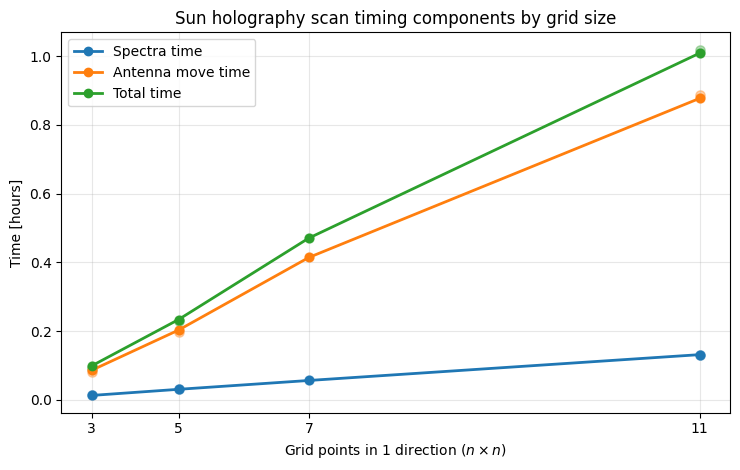
\includegraphics[width=0.82\linewidth]{Images/scan_time_measured.png}
    \caption{Measured scan timing components from the log files. The spectra time is calculated from the RFSoC spectra count multiplied by 3.56 s. The antenna move time is the difference between the total log time and the spectra time.}
    \label{fig:scan-time-measured}
\end{figure}

For the extrapolated scans, the grid is divided into square shells. For an odd grid size $G$, the maximum shell number is

\begin{equation}
K = \frac{G - 1}{2}.
\end{equation}

The center point is shell 0. For shells $k \geq 1$, the number of points in each shell is

\begin{equation}
n_k = 8k .
\end{equation}

The weighted scan uses shell weights

\begin{equation}
w_k = k^2 ,
\end{equation}

with the center shell assigned weight $w_0 = 1$. The total weighted spectra count is

\begin{equation}
N_{\mathrm{spectra}} =
n_0 w_0 + \sum_{k=1}^{K} n_k w_k + (G + 1),
\end{equation}

where $(G+1)$ accounts for the boresight spectra.

The antenna move time is not scaled by the shell weights, since repeated spectra at the same grid point increase integration time but do not require additional antenna movement. Instead, the measured antenna move times for $G=3,5,7,11$ are used directly. For larger grids, the antenna move time is extrapolated using a linear fit in $G^2$:

\begin{equation}
t_{\mathrm{move}}(G) = aG^2 + b .
\end{equation}

The main functions used for the calculation are shown below.

\begin{lstlisting}[language=Python]
def shell_point_counts(grid_size):
    max_shell = grid_size // 2
    return np.array([1] + [8 * shell for shell in range(1, max_shell + 1)])
\end{lstlisting}

This function returns the number of points in each square shell. Shell 0 contains one point, and shell $k$ contains $8k$ points.

\begin{lstlisting}[language=Python]
def weighted_spectra_count(grid_size):
    max_shell = grid_size // 2

    points_per_shell = shell_point_counts(grid_size)
    shell_weights = np.arange(1, max_shell + 1) ** 2
    weights_by_shell = np.concatenate(([1], shell_weights))

    grid_spectra = np.sum(points_per_shell * weights_by_shell)
    boresight_spectra = grid_size + 1

    return grid_spectra + boresight_spectra
\end{lstlisting}

This function computes the total number of spectra for a weighted shell scan. The shell weights are $[1,2,\ldots,K]^2$, with shell 0 assigned weight 1. The boresight spectra are added separately as $G+1$.

\begin{lstlisting}[language=Python]
known_grid_sizes = np.array([3, 5, 7, 11])
known_move_times_s = np.array([
    309.72,
    730.64,
    1491.08,
    3157.52,
])

move_fit = np.poly1d(
    np.polyfit(known_grid_sizes**2, known_move_times_s, deg=1)
)
\end{lstlisting}

This code fits the measured antenna move times as a linear function of $G^2$. The fit is only used for grid sizes larger than those measured in the logs.

\begin{lstlisting}[language=Python]
def antenna_move_time_s(grid_size):
    match = np.where(known_grid_sizes == grid_size)[0]
    if len(match):
        return float(known_move_times_s[match[0]])

    return float(move_fit(grid_size**2))
\end{lstlisting}

This function returns the measured antenna move time for $G=3,5,7,11$. For larger grid sizes, it evaluates the $G^2$ fit.

\begin{lstlisting}[language=Python]
def spectra_time_s(grid_size):
    return weighted_spectra_count(grid_size) * SPECTRUM_TIME_S

def total_scan_time_s(grid_size):
    return spectra_time_s(grid_size) + antenna_move_time_s(grid_size)
\end{lstlisting}

These final functions convert the spectra count into time and then add the antenna move time to estimate the full scan duration. Figure~\ref{fig:scan-time-extrapolated} shows the resulting scan time estimate for the weighted shell scheme. The solid blue curve uses measured log-derived move times. The dashed orange curve shows the extrapolated estimates for larger grids.

\begin{figure}[H]
    \centering
    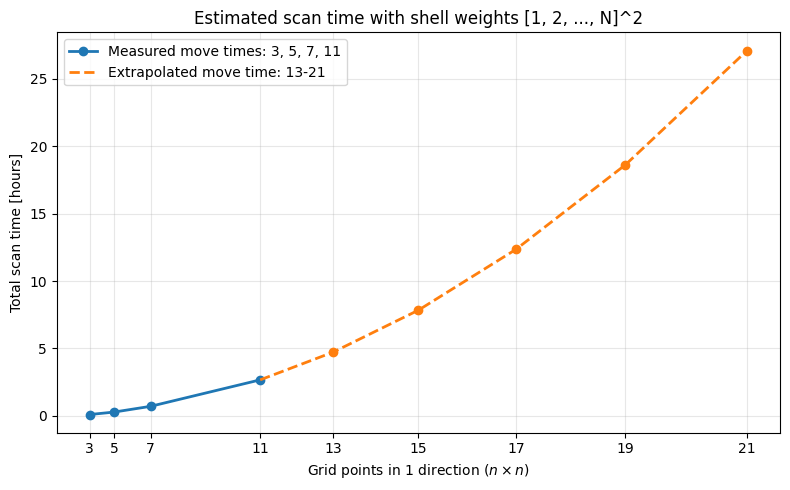
\includegraphics[width=0.82\linewidth]{Images/scan_time_extrapolat.png}
    \caption{Estimated total scan time for weighted shell scans using weights $[1,2,\ldots,K]^2$. Measured antenna move times are used for $G=3,5,7,11$, and larger grid sizes are extrapolated using a linear fit in $G^2$.}
    \label{fig:scan-time-extrapolated}
\end{figure}

Following the current weighting scheme, the biggest map we can make due to time constraints is 13x13. 
\subsection{Making Surface Error Maps 1: Accounting for Geometric Delay \& Cable Length Differences}
\subsubsection{Consideration 1: Geometric Delay Correction, Fringe Stopping}

In an interferometer, a signal arriving from a source reaches the two antennas at slightly different times. This time difference is called the \textit{geometric delay}. If this delay is not corrected, the measured cross-correlation contains a rapidly varying phase term. This phase variation is especially important for a bright moving source such as the Sun because the projected baseline changes with time as the Earth rotates. The purpose of fringe stopping is to remove this known geometric phase term so that the visibility phase is referenced to the source direction.
\begin{figure}[H]
    \centering
    \safeincludegraphics[width=\linewidth]{Images/no_delay_corr.png}
    \caption{Time vs Phase of AD and BC cross correlations without geometric delay accounted for.}
    \label{fig:no_delay_corr}
\end{figure}
Before applying the geometric delay correction, the measured cross-correlation phase is not expected to remain fixed in time. Figure~\ref{fig:no_delay_corr} shows the phase of the AD and BC cross-correlations near $1.800~\mathrm{GHz}$ as a function of time, including both grid point measurements and boresight returns. The phases scatter and drift over time because the projected antenna baseline toward the Sun changes as the Sun moves across the sky. This changing projection produces a time-dependent geometric delay, which appears as a frequency-dependent and time-dependent phase term in the visibility. Therefore, even when the antennas return to boresight, the measured phase can differ from the previous boresight phase if the geometric delay has not been removed. This motivates the fringe-stopping correction: we compute the expected geometric delay from the baseline vector and the Sun direction, then rotate each complex visibility by the corresponding phase factor so that the visibility phase is referenced to the Sun. \\

\noindent The notebook performs this correction using two vectors: the \textit{baseline vector} between the antennas and the \textit{source direction vector} pointing toward the Sun. The code figures out these vectors in two different ways. First, the antenna latitudes and longitudes are passed to \texttt{EarthLocation}. Astropy converts these geodetic coordinates into Earth-fixed Cartesian coordinates in the ITRS/ITRF frame. This gives one position vector for the North antenna and one position vector for the South antenna,
\begin{equation}
\mathbf{r}_{N} = (x_N,y_N,z_N),
\end{equation}
\begin{equation}
\mathbf{r}_{S} = (x_S,y_S,z_S).
\end{equation}
The antenna baseline vector is then found by subtracting these two Earth-fixed position vectors,
\begin{equation}
\mathbf{b} = \mathbf{r}_{N} - \mathbf{r}_{S}.
\end{equation}
Second, the code uses the Unix \texttt{timestamp}s for each spectrum to compute the apparent position of the Sun at that exact time using \texttt{get\_sun(obs\_times)}. The Sun position is then transformed into the same Earth-fixed ITRS frame as the baseline. This gives a time-dependent Sun vector,
\begin{equation}
\mathbf{s}(t) = (s_x(t),s_y(t),s_z(t)).
\end{equation}
Since the delay calculation only needs the direction to the Sun and not the Sun--Earth distance, the code normalizes this vector to make a unit direction vector,
\begin{equation}
\hat{\mathbf{s}}(t)=\frac{\mathbf{s}(t)}{|\mathbf{s}(t)|}.
\label{eq:source-unit-vector}
\end{equation}
Thus, the delay correction is built from one fixed vector, $\mathbf{b}$, describing the antenna separation, and one time-dependent unit vector, $\hat{\mathbf{s}}(t)$, describing where the Sun is in the sky in the same coordinate system.

The relevant code begins by defining the speed of light and the antenna locations:

\begin{lstlisting}[language=Python]
import astropy.units as u
from astropy.coordinates import (
EarthLocation, SkyCoord, ITRS, get_sun)
from astropy.time import Time

c_light = 2.998e8   # m/s

# --- Antenna locations ----------------------------------------

loc_n = EarthLocation(lat=lat_n * u.deg, lon=lon_n * u.deg, height=0 * u.m)
loc_s = EarthLocation(lat=lat_s * u.deg, lon=lon_s * u.deg, height=0 * u.m)
\end{lstlisting}

Here, \texttt{loc\_n} and \texttt{loc\_s} are the positions of the North and South antennas. These are specified using geodetic latitude and longitude, then converted internally by \texttt{astropy} into Earth-centered coordinates.

The baseline vector is then computed as the difference between the North antenna position and the South antenna position:

\begin{lstlisting}[language=Python]

# Baseline N - S in ITRF (metres)

b_itrf = (loc_n.get_itrs().cartesian.xyz.to(u.m).value
- loc_s.get_itrs().cartesian.xyz.to(u.m).value)

print(f"Baseline N-S (ITRF, metres): {b_itrf}")
print(f"Baseline length: {np.linalg.norm(b_itrf):.3f} m")
\end{lstlisting}

Mathematically, this is
\begin{equation}
\mathbf{b} = \mathbf{r}_{N} - \mathbf{r}_{S},
\end{equation}
where $\mathbf{r}_{N}$ is the Earth-fixed position vector of the North antenna, $\mathbf{r}_{S}$ is the Earth-fixed position vector of the South antenna, and $\mathbf{b}$ is the baseline vector pointing from the South antenna to the North antenna. The baseline length is
\begin{equation}
|\mathbf{b}| = \sqrt{b_x^2 + b_y^2 + b_z^2}.
\end{equation}

Since the baseline vector is computed in the Earth-fixed ITRS/ITRF coordinate frame, the source direction must also be expressed in the same frame. The notebook gets the Sun's position at every \texttt{timestamp}:

\begin{lstlisting}[language=Python]

# --- Sun direction at each timestamp --------------------------

obs_times = Time(sys_ts, format="unix")
sun_coords = get_sun(obs_times)   # GCRS SkyCoord
\end{lstlisting}

Here, \texttt{sys\_ts} contains the Unix \texttt{timestamp}s of the spectra. The code converts these into an \texttt{astropy} \texttt{Time} object and then uses \texttt{get\_sun()} to compute the apparent position of the Sun at each observation time.

The Sun coordinates are then transformed into the ITRS frame:

\begin{lstlisting}[language=Python]

# Transform to ITRS for geometric delay computation

sun_itrs = sun_coords.transform_to(ITRS(obstime=obs_times))
s_xyz = sun_itrs.cartesian.xyz.value   # (3, n_spec_total)
\end{lstlisting}

This gives a vector pointing from the Earth toward the Sun at each \texttt{timestamp}. Because only the direction matters for geometric delay, the vector is normalized to make a unit vector:

\begin{lstlisting}[language=Python]

# Normalise to unit vectors

s_norm = np.sqrt(np.sum(s_xyz**2, axis=0))
s_xyz = s_xyz / s_norm[np.newaxis, :]
\end{lstlisting}

Mathematically, if the unnormalized Sun vector is $\mathbf{s}(t)$, the normalized direction vector is
The normalized Sun direction is given by Eq.~\eqref{eq:source-unit-vector}.

The normalization factor is
\begin{equation}
|\mathbf{s}(t)| = \sqrt{s_x(t)^2 + s_y(t)^2 + s_z(t)^2}.
\end{equation}

The geometric delay is the projection of the baseline vector onto the source direction, divided by the speed of light:

\begin{lstlisting}[language=Python]
tau_g = (b_itrf @ s_xyz) / c_light   # (n_spec_total,) seconds

print(f"Geometric delay range: {tau_g.min()*1e9:.3f} -- "
f"{tau_g.max()*1e9:.3f} ns")
\end{lstlisting}

The corresponding equation is
\begin{equation}
\tau_g(t) = \frac{\mathbf{b} \cdot \hat{\mathbf{s}}(t)}{c},
\end{equation}
where $c$ is the speed of light. Expanding the dot product,
\begin{equation}
\tau_g(t) = \frac{
b_x \hat{s}_x(t) +
b_y \hat{s}_y(t) +
b_z \hat{s}_z(t)
}{c}.
\end{equation}

This quantity tells us the expected arrival-time difference between the two antennas for radiation coming from the Sun. If $\tau_g > 0$, the sign convention used by the code says that the wavefront reaches one antenna later than the other according to the baseline definition $\mathbf{b} = \mathbf{r}_{N} - \mathbf{r}_{S}$.

A time delay corresponds to a frequency-dependent phase. For a monochromatic signal with frequency $\nu$, a delay $\tau_g$ produces a phase
\begin{equation}
\phi_g(t,\nu) = 2\pi \nu \tau_g(t).
\end{equation}

Therefore, the geometric phase term is
\begin{equation}
e^{i2\pi \nu \tau_g(t)}.
\end{equation}

In the notebook, the frequencies are first converted from MHz to Hz:

\begin{lstlisting}[language=Python]
freqs_Hz = freqs * 1e6
\end{lstlisting}

The phase correction is then constructed as a two-dimensional array, with one axis for time and one axis for frequency:

\begin{lstlisting}[language=Python]
phase_corr = np.exp(2j * np.pi * tau_g[:, None] * freqs_Hz[None, :])
\end{lstlisting}

This corresponds to
\begin{equation}
\exp\left[i2\pi \nu \tau_g(t)\right].
\end{equation}

The indexing in the code makes this correction apply to every \texttt{timestamp} and every frequency channel. The term \texttt{tau\_g[:, None]} gives an array with shape $(N_t, 1)$, while \texttt{freqs\_Hz[None, :]} gives an array with shape $(1, N_\nu)$. Multiplying them produces a correction array with shape $(N_t, N_\nu)$.

Before applying the correction, the notebook selects the desired cross-correlation products:

\begin{lstlisting}[language=Python]
# --- Apply fringestopping to cross-corr products -------------

cross_keys = list(CROSS_PAR.keys())
cross_idx  = [CROSS_PAR[k] for k in cross_keys]

raw_cross = spectra_raw[:, cross_idx, :].copy()
\end{lstlisting}

Here, \texttt{CROSS\_PAR} maps baseline labels to their indices in the correlator output. For example, if the desired cross-correlations are AD and BC, then

\begin{lstlisting}[language=Python]
CROSS_PAR = {"AD": 3, "BC": 5}
\end{lstlisting}

and the notebook extracts those products from \texttt{spectra\_raw}. If the original raw cross-correlation is written as
\begin{equation}
V_{\rm raw}(t,\nu),
\end{equation}
then after selecting the relevant products, the notebook applies the fringe-stopping phasor:

\begin{lstlisting}[language=Python]
for ci in range(len(cross_keys)):
    raw_cross[:, ci, :] *= phase_corr
\end{lstlisting}

Mathematically, this means
\begin{equation}
V_{\rm fs}(t,\nu) = V_{\rm raw}(t,\nu)\exp\left[i2\pi \nu \tau_g(t)\right],
\end{equation}
where $V_{\rm fs}$ is the fringe-stopped visibility.

The reason this works is that the raw visibility contains a geometric phase term. With the sign convention used in the notebook, the raw visibility can be written approximately as
\begin{equation}
V_{\rm raw}(t,\nu) = V_0(t,\nu)\exp\left[-i2\pi \nu \tau_g(t)\right],
\end{equation}
where $V_0(t,\nu)$ is the visibility after removing the geometric phase. Multiplying by the correction gives
\begin{equation}
V_0(t,\nu)\exp\left[-i2\pi \nu \tau_g(t)\right]\exp\left[i2\pi \nu \tau_g(t)\right].
\end{equation}

The two exponential terms cancel:
\begin{equation}
V_{\rm fs}(t,\nu) = V_0(t,\nu).
\end{equation}

Thus, fringe stopping removes the phase winding caused by the changing geometric delay. Before the correction, the phase of the visibility changes with time and frequency according to
\begin{equation}
\phi_{\rm raw}(t,\nu) \approx \phi_0(t,\nu) - 2\pi \nu \tau_g(t).
\end{equation}

After the correction, the phase becomes
\begin{equation}
\phi_{\rm fs}(t,\nu) \approx \phi_0(t,\nu).
\end{equation}

Therefore, if the correction is working, the phase should be much flatter versus time for a fixed frequency channel, and much flatter versus frequency for a fixed time sample. Equivalently, a waterfall plot of phase versus time and frequency should show that the drifting fringe pattern has been removed or significantly reduced.

The final corrected cross-correlation array, called \texttt{raw\_cross} in the notebook after the multiplication, is then used in the next stage of the analysis for bandpass calibration. The essential sequence is therefore:

\begin{equation}
\mathbf{b} = \mathbf{r}_{N} - \mathbf{r}_{S}
\end{equation}

\begin{equation}
\hat{\mathbf{s}}(t) = \frac{\mathbf{s}(t)}{|\mathbf{s}(t)|}
\end{equation}

\begin{equation}
\tau_g(t) = \frac{\mathbf{b}\cdot\hat{\mathbf{s}}(t)}{c}
\end{equation}

\begin{equation}
\exp\left[i2\pi\nu\tau_g(t)\right]
\end{equation}

\begin{equation}
V_{\rm fs}(t,\nu) = V_{\rm raw}(t,\nu)\exp\left[i2\pi\nu\tau_g(t)\right]
\end{equation}
This gives us a flat phase that is no longer a function of time. Hence, a flat line on the the plot though not necessarily centered at 0 due to the different fiber optic cable lengths of the antennas which will vary as a function of wavelength.

\begin{figure}[H]
    \centering
    \safeincludegraphics[width=0.9\linewidth]{Images/Before_cable_corr.png}
    \caption{Phase versus time for the AD and BC baselines after applying only the geometric fringe-stopping correction. The raw grid and boresight measurements are shown together with the geometrically corrected points. At this stage, residual phase structure remains because fixed instrumental delays, such as cable length differences, are not yet removed.}
    \label{fig:before_cable_corr}
\end{figure}

\subsubsection{Consideration 2: Cable Length Differences}
After applying the geometric fringe-stopping correction based on the Sun ephemeris and baseline geometry, a residual phase drift remained in the visibilities. This residual term is attributed to differential electrical path lengths, such as unequal cable lengths and other slowly varying instrumental phase offsets. In other words, geometric delay removal alone is not sufficient to fully flatten the boresight phase. This can be seen in Figure~\ref{fig:before_cable_corr}, where the phases still show a clear time-dependent structure even after the geometric correction has been applied.

We write the measured phase as
\begin{equation}
\phi_{\mathrm{meas}}(t) = \phi_{\mathrm{geo}}(t) + \phi_{\mathrm{cable}}(t) + \phi_{\mathrm{noise}}(t),
\end{equation}
where $\phi_{\mathrm{geo}}(t)$ is the predicted geometric fringe phase, $\phi_{\mathrm{cable}}(t)$ is the residual instrumental phase term, and $\phi_{\mathrm{noise}}(t)$ represents measurement noise. After removing the geometric contribution, the remaining phase is
\begin{equation}
\phi_{\mathrm{res}}(t) = \phi_{\mathrm{meas}}(t) - \phi_{\mathrm{geo}}(t).
\end{equation}

To model this residual term, we use \textbf{three different types of fitting} applied to the boresight phase as a function of time:
\begin{enumerate}
    \item an anchored cosine fit,
    \item a linear fit,
    \item an $n$th-degree polynomial fit.
\end{enumerate}

These three fitting choices provide flexibility in describing different forms of slowly varying instrumental phase drift. The anchored cosine fit is useful when the residual phase shows oscillatory behavior, the linear fit captures a simple monotonic drift, and the polynomial fit allows a more general smooth trend. The fitted residual phase model, denoted $\theta(t)$, is then used to correct both the grid-point visibility at time $t_2$ and the corresponding boresight reference visibility at time $t_1$. The correction factor is
\begin{equation}
\frac{e^{-i\theta(t_2)}}{e^{-i\theta(t_1)}}.
\end{equation}

The final beam estimate is therefore written as
\begin{equation}
B(x,y) =
\frac{V(x,y,t_2)}{V(0,0,t_1)}
\frac{e^{+i 2\pi \tau_g(t_2)\nu}}{e^{+i 2\pi \tau_g(t_1)\nu}}
\frac{e^{-i\theta(t_2)}}{e^{-i\theta(t_1)}},
\end{equation}
where $\tau_g(t)$ is the predicted geometric delay and $\nu$ is the selected observing frequency.

In the notebook, the residual phase correction is implemented as
\begin{lstlisting}[language=Python]
theta_t2 = evaluate_path_phase_fit(cross_name, grid_t)
theta_t1 = evaluate_path_phase_fit(cross_name, boresight_t)[previous_boresight]

path_corr_t2 = np.exp(-1j * theta_t2)
path_corr_t1 = np.exp(-1j * theta_t1)

beam = (v_grid / v_boresight) \
    * (geom_corr_t2 / geom_corr_t1) \
    * (path_corr_t2 / path_corr_t1)
\end{lstlisting}

After this additional correction is applied, the residual instrumental phase drift is substantially reduced. Figure~\ref{fig:after_cable_corr} shows that the boresight points are driven much closer to zero phase, while the grid measurements become better aligned with the corrected reference. This produces a more stable phase calibration and leads to a cleaner beam reconstruction.

\begin{figure}[H]
    \centering
    \safeincludegraphics[width=0.9\linewidth]{Images/After_cable_corr.png}
    \caption{Phase versus time for the AD and BC baselines after applying both the geometric fringe-stopping correction and the residual cable-length correction. The residual instrumental phase drift is modeled with an empirical fit, using one of three fitting options: anchored cosine, linear, or polynomial. After this additional correction, the boresight points are driven much closer to zero phase, and the grid measurements are correspondingly better aligned for beam reconstruction.}
    \label{fig:after_cable_corr}
\end{figure}
\subsubsection{Fourier Transforming the Beam to the Aperture}

After applying the geometric delay and different cable lengths correction, the next step is to convert the measured beam maps into aperture-plane illumination maps. The measured beam is sampled as a function of angular offset on the sky, while the desired aperture illumination is a function of physical position across the dish. These two planes are Fourier pairs. Therefore, once the complex beam is measured over cross-elevation and elevation offsets, the aperture illumination can be reconstructed by taking an inverse Fourier transform of the beam.

Figure~\ref{fig:beam_maps_ad_bc} shows the measured beam amplitude for the AD and BC cross-correlations at $1.000~\mathrm{GHz}$. The black points show the sampled grid positions. The beam is strongest near boresight and falls off toward larger angular offsets. This beam map is the input to the aperture reconstruction.

\begin{figure}[H]
    \centering
    \safeincludegraphics[width=\linewidth]{Images/Beam.png}
    \caption{Measured beam amplitude maps for the AD and BC cross-correlations at $1.000~\mathrm{GHz}$. The black points show the sampled scan grid positions.}
    \label{fig:beam_maps_ad_bc}
\end{figure}

Let the measured complex beam be

\begin{equation}
    B(\theta_{\mathrm{xel}}, \theta_{\mathrm{el}}),
\end{equation}

where $\theta_{\mathrm{xel}}$ is the cross-elevation offset and $\theta_{\mathrm{el}}$ is the elevation offset. These angular coordinates are converted into Fourier-plane coordinates using

\begin{equation}
    u = \frac{\sin(\theta_{\mathrm{xel}})}{\lambda},
\end{equation}

and

\begin{equation}
    v = \frac{\sin(\theta_{\mathrm{el}})}{\lambda}.
\end{equation}

Here, $\lambda$ is the observing wavelength. The coordinates $u$ and $v$ have units of inverse meters and are the spatial-frequency coordinates conjugate to the aperture-plane coordinates $x$ and $y$.

The forward relationship between aperture illumination and beam is

\begin{equation}
    B(u,v)
    =
    \int_{-\infty}^{\infty}
    \int_{-\infty}^{\infty}
    A(x,y)
    e^{-i2\pi(ux+vy)}
    \, dx\,dy,
\end{equation}

where $A(x,y)$ is the complex aperture illumination. Therefore, to recover the aperture illumination from the measured beam, we use the inverse Fourier transform:

\begin{equation}
    A(x,y)
    =
    \int_{-\infty}^{\infty}
    \int_{-\infty}^{\infty}
    B(u,v)
    e^{+i2\pi(ux+vy)}
    \, du\,dv.
\end{equation}

In discrete form, the inverse transform is approximated by

\begin{equation}
    A(x_n,y_m)
    \approx
    \Delta u \Delta v
    \sum_{p=0}^{N_u-1}
    \sum_{q=0}^{N_v-1}
    B(u_p,v_q)
    e^{+i2\pi(u_p x_n + v_q y_m)}.
\end{equation}

The code implements this operation using a two-dimensional inverse FFT:

\begin{lstlisting}
def aperture_axes_from_angle_grid(xel_deg_values, el_deg_values, wavelength):
    xel_rad = np.deg2rad(np.asarray(xel_deg_values, dtype=float))
    el_rad = np.deg2rad(np.asarray(el_deg_values, dtype=float))

    u = np.sin(xel_rad) / wavelength
    v = np.sin(el_rad) / wavelength

    du = np.nanmedian(np.diff(np.sort(u)))
    dv = np.nanmedian(np.diff(np.sort(v)))

    aperture_x = np.fft.fftshift(np.fft.fftfreq(len(u), d=du))
    aperture_y = np.fft.fftshift(np.fft.fftfreq(len(v), d=dv))

    return aperture_x, aperture_y, u, v
\end{lstlisting}

The angular scan grid is first converted into the Fourier coordinates $u$ and $v$. The grid spacings are

\begin{equation}
    \Delta u
    =
    \mathrm{median}
    \left[
    u_{p+1} - u_p
    \right],
\end{equation}

and

\begin{equation}
    \Delta v
    =
    \mathrm{median}
    \left[
    v_{q+1} - v_q
    \right].
\end{equation}

The aperture axes are then generated with \texttt{np.fft.fftfreq}. Since $u$ and $v$ have units of inverse meters, their Fourier-conjugate coordinates have units of meters. Therefore, the reconstructed aperture maps are plotted in physical aperture coordinates $(x,y)$.

The aperture reconstruction is performed by

\begin{lstlisting}
def beam_to_aperture_illumination_fft(beam_image, xel_values, el_values, wavelength_m):
    beam_image = np.asarray(beam_image, dtype=complex)

    aperture_x, aperture_y, u, v = aperture_axes_from_angle_grid(
        xel_values,
        el_values,
        wavelength_m,
    )

    du = np.nanmedian(np.diff(np.sort(u)))
    dv = np.nanmedian(np.diff(np.sort(v)))

    aperture = np.fft.fftshift(
        np.fft.ifft2(
            np.fft.ifftshift(beam_image)
        )
    )

    aperture *= beam_image.shape[0] * beam_image.shape[1] * du * dv

    return aperture_x, aperture_y, aperture
\end{lstlisting}

The main transform line is

\begin{lstlisting}
aperture = np.fft.fftshift(np.fft.ifft2(np.fft.ifftshift(beam_image)))
\end{lstlisting}

The inner \texttt{ifftshift} moves the zero-offset beam sample to the array convention expected by \texttt{ifft2}. The \texttt{ifft2} then performs the two-dimensional inverse Fourier transform. The outer \texttt{fftshift} moves the reconstructed aperture back to a centered coordinate system for plotting.

Because NumPy's inverse FFT includes a normalization of $1/(N_uN_v)$, the code multiplies the result by $N_uN_v\Delta u\Delta v$:

\begin{equation}
    A(x,y)
    \approx
    N_uN_v\Delta u\Delta v
    \,
    \mathrm{fftshift}
    \left[
    \mathrm{ifft2}
    \left(
    \mathrm{ifftshift}
    \left[
    B(u,v)
    \right]
    \right)
    \right].
\end{equation}

This normalization makes the discrete sum match the continuous inverse Fourier transform convention,

\begin{equation}
    A(x,y)
    =
    \int
    \int
    B(u,v)
    e^{+i2\pi(ux+vy)}
    \,du\,dv.
\end{equation}

Figure~\ref{fig:aperture_1p8_ad_bc} shows the reconstructed aperture illumination at $1.800041~\mathrm{GHz}$. The left column shows the normalized aperture amplitude in decibels, while the right column shows the aperture phase in radians. The dashed circle marks the approximate physical dish diameter. The amplitude maps show how strongly different parts of the dish are illuminated. The phase maps show the phase structure across the aperture, which can contain contributions from surface errors, pointing errors, instrumental phase offsets, and residual calibration errors.

\begin{figure}[H]
    \centering
    \safeincludegraphics[width=\linewidth]{Images/Apeture@1pt8.png}
    \caption{Reconstructed aperture illumination for AD and BC at $1.800041~\mathrm{GHz}$. The left panels show normalized aperture amplitude in dB, and the right panels show aperture phase in radians. The dashed circle marks the approximate dish aperture.}
    \label{fig:aperture_1p8_ad_bc}
\end{figure}

The aperture amplitude is computed from the complex aperture illumination as

\begin{equation}
    |A(x,y)|
    =
    \sqrt{
    \mathrm{Re}[A(x,y)]^2
    +
    \mathrm{Im}[A(x,y)]^2
    },
\end{equation}

and the aperture phase is

\begin{equation}
    \phi_A(x,y)
    =
    \arg[A(x,y)].
\end{equation}

The normalized aperture amplitude in decibels is

\begin{equation}
    A_{\mathrm{dB}}(x,y)
    =
    20\log_{10}
    \left[
    \frac{|A(x,y)|}{\max |A(x,y)|}
    \right].
\end{equation}

This normalization sets the brightest aperture pixel to $0~\mathrm{dB}$ and shows the illumination falloff toward the edge of the dish.

To reduce frequency-dependent noise and make the stable aperture illumination easier to see, aperture maps from multiple frequencies can be averaged. For each aperture pixel, the average aperture amplitude is computed from the maps at $0.95~\mathrm{GHz}$, $1.4~\mathrm{GHz}$, and $1.8~\mathrm{GHz}$:

\begin{equation}
A_{\mathrm{avg}}(x,y)
=
\frac{
A_{0.95}(x,y)
+
A_{1.4}(x,y)
+
A_{1.8}(x,y)
}{3}.
\end{equation}

Here, $A_{0.95}(x,y)$, $A_{1.4}(x,y)$, and $A_{1.8}(x,y)$ are the reconstructed aperture amplitudes at the three different frequencies, evaluated on the same interpolated aperture grid. This averaging is done pixel-by-pixel, so each location in the aperture plane is averaged only with the corresponding location in the other frequency maps. For the real map, I will average ~100 frequency channels, while avoiding 0.85 and 1.8 GHz as they are areas with high RFI.

Figure~\ref{fig:averaged_aperture_ad_bc} shows the average aperture amplitude over the interpolated frequency maps. The averaged maps for AD and BC are smoother than any individual map and show the main aperture illumination pattern more clearly. The strongest illumination is near the center of the dish and decreases toward the edge, as expected for a tapered aperture illumination. The dashed circle again marks the approximate dish diameter.

\begin{figure}[H]
    \centering
    \safeincludegraphics[width=\linewidth]{Images/Averaged_apeture.png}
    \caption{Average aperture amplitude over interpolated frequency maps at $0.95~\mathrm{GHz}$, $1.40~\mathrm{GHz}$, and $1.80~\mathrm{GHz}$. The average is computed pixel-by-pixel using $A_{\mathrm{avg}}(x,y) = [A_{0.95}(x,y)+A_{1.4}(x,y)+A_{1.8}(x,y)]/3$.}
    \label{fig:averaged_aperture_ad_bc}
\end{figure}

This Fourier-transform step connects the measured sky response to the physical antenna aperture. The beam maps show how the antenna responds as a function of angular offset from the Sun, while the aperture maps show where the received electric field is distributed across the dish. In this way, holography converts angular beam measurements into a spatial diagnostic of the antenna aperture.
\subsubsection{Consideration 3: Phase Gradient Due to Pointing Error}

As shown previously in Figure~\ref{fig:aperture_1p8_ad_bc}, the reconstructed aperture phase contains a pronounced linear gradient across the reflector. This gradient is consistent with a residual pointing error: by the Fourier shift theorem, an angular displacement of the measured far-field beam from the assumed boresight direction produces a linear phase ramp in the aperture plane.

The measured complex aperture illumination can be written as
\begin{equation}
A_{\mathrm{meas}}(x,y)
=
\left|A_{\mathrm{meas}}(x,y)\right|
\exp\left[i\phi_{\mathrm{meas}}(x,y)\right],
\end{equation}
where $\left|A_{\mathrm{meas}}(x,y)\right|$ is the aperture amplitude and $\phi_{\mathrm{meas}}(x,y)$ is its measured phase.

A first-order pointing offset produces an approximately linear aperture phase:
\begin{equation}
\phi_{\mathrm{point}}(x,y)
=
\phi_0 + g_x x + g_y y,
\end{equation}
where $\phi_0$ is a constant phase offset, while $g_x$ and $g_y$ are the phase gradients in the cross-elevation and elevation directions, respectively, in units of radians per metre.

Under the small-angle approximation, the fitted phase gradients are related to the direction-cosine pointing offsets by
\begin{equation}
\Delta l = \frac{\lambda g_x}{2\pi},
\qquad
\Delta m = \frac{\lambda g_y}{2\pi},
\end{equation}
where $\lambda$ is the observing wavelength. The signs of these expressions depend on the Fourier-transform convention used to reconstruct the aperture.

The coefficients $\phi_0$, $g_x$, and $g_y$ were obtained by fitting a plane to the aperture phase. Only finite samples within the physical dish aperture were included in the fit. The linear model can be written in matrix form as
\begin{equation}
\begin{bmatrix}
1 & x_1 & y_1 \\
1 & x_2 & y_2 \\
\vdots & \vdots & \vdots \\
1 & x_N & y_N
\end{bmatrix}
\begin{bmatrix}
\phi_0 \\
g_x \\
g_y
\end{bmatrix}
\simeq
\begin{bmatrix}
\phi_1 \\
\phi_2 \\
\vdots \\
\phi_N
\end{bmatrix}.
\end{equation}

Because the aperture phase is wrapped to the interval $[-\pi,\pi)$, the fit residual was evaluated using wrapped phase differences:
\begin{equation}
r_n
=
\arg\left[
\exp\left(
i\left[
\phi_n-\phi_{\mathrm{point}}(x_n,y_n)
\right]
\right)
\right].
\end{equation}
This prevents samples immediately below $-\pi$ and immediately above $+\pi$ from being treated as though they differ by approximately $2\pi$.

A representative implementation of the wrapped linear phase fit is shown below.

\begin{lstlisting}[language=Python]
from scipy.optimize import least_squares


def wrap_phase(phase):
    return np.angle(np.exp(1j * phase))


def fit_aperture_phase_plane(
    aperture,
    aperture_x,
    aperture_y,
    dish_radius,
):
    X, Y = np.meshgrid(aperture_x, aperture_y)

    phase = np.angle(aperture)
    amplitude = np.abs(aperture)

    valid = (
        np.isfinite(aperture.real)
        & np.isfinite(aperture.imag)
        & (X**2 + Y**2 <= dish_radius**2)
        & (amplitude > 0)
    )

    x_fit = X[valid]
    y_fit = Y[valid]
    phase_fit = phase[valid]

    # Start with the circular mean phase and zero gradients.
    phi0_initial = np.angle(np.mean(np.exp(1j * phase_fit)))
    initial = np.array([phi0_initial, 0.0, 0.0])

    def residual(coefficients):
        phi0, gx, gy = coefficients
        phase_model = phi0 + gx * x_fit + gy * y_fit
        return wrap_phase(phase_fit - phase_model)

    result = least_squares(
        residual,
        initial,
        max_nfev=100000,
    )

    phi0, gx, gy = result.x
    fitted_phase_plane = phi0 + gx * X + gy * Y

    corrected_aperture = (
        aperture * np.exp(-1j * fitted_phase_plane)
    )

    corrected_phase = np.angle(corrected_aperture)
    corrected_residual = corrected_phase[valid]
    corrected_rms = np.sqrt(
        np.mean(corrected_residual**2)
    )

    return {
        "corrected_aperture": corrected_aperture,
        "corrected_phase": corrected_phase,
        "fitted_phase_plane": fitted_phase_plane,
        "coefficients": result.x,
        "rms_rad": corrected_rms,
        "valid": valid,
    }
\end{lstlisting}

The fitted phase plane was removed directly from the complex aperture illumination:
\begin{equation}
A_{\mathrm{corr}}(x,y)
=
A_{\mathrm{meas}}(x,y)
\exp\left[
-i\left(
\phi_0+g_xx+g_yy
\right)
\right].
\end{equation}
The corrected aperture phase is therefore
\begin{equation}
\phi_{\mathrm{corr}}(x,y)
=
\arg\left[A_{\mathrm{corr}}(x,y)\right].
\end{equation}

This operation changes only the phase of the complex aperture; it does not alter its measured amplitude:
\begin{equation}
\left|A_{\mathrm{corr}}(x,y)\right|
=
\left|A_{\mathrm{meas}}(x,y)\right|.
\end{equation}

Figure~\ref{fig:removing_phase_gradient} shows the fitted phase planes and corrected aperture phases for the AD and BC correlations. The left-hand plots show the wrapped phase before correction together with the fitted plane. The middle plots show the aperture phase after removing the fitted linear gradient, while the right-hand plots show the corrected phase on the two-dimensional aperture grid.

\begin{figure}[H]
    \centering
    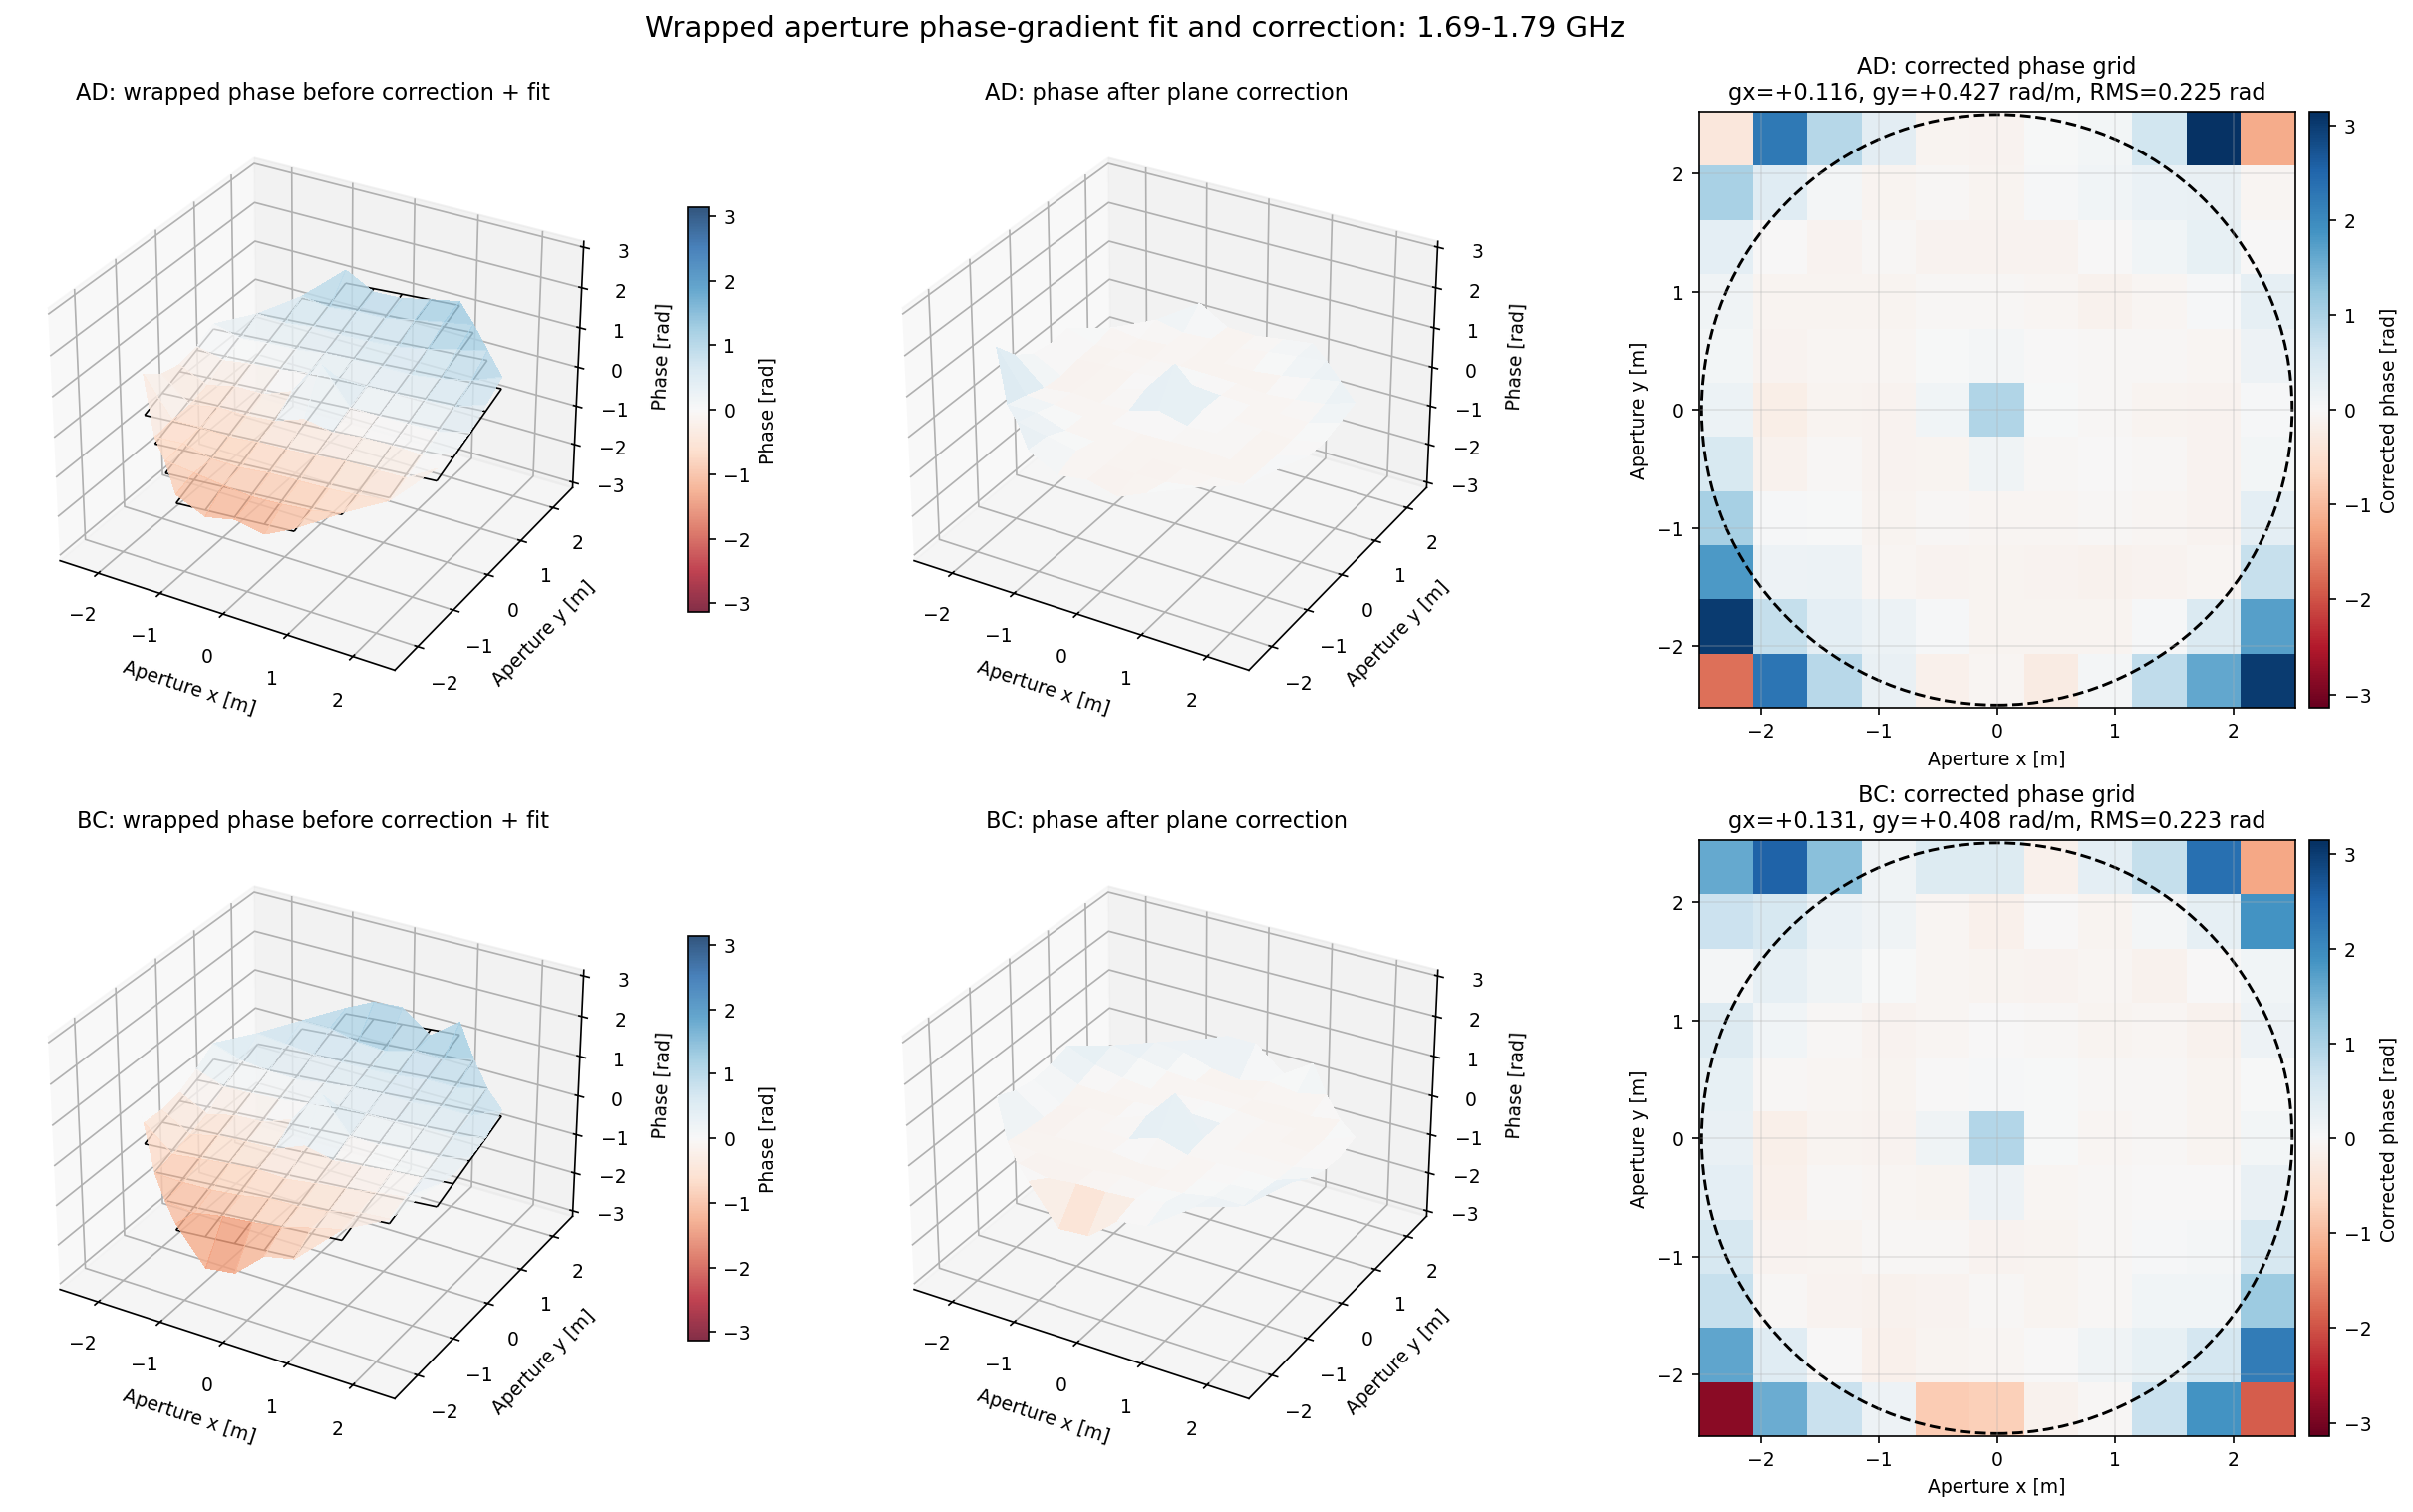
\includegraphics[width=\linewidth]
    {Images/removing_phase_gradient.png}
    \caption{Removal of the linear aperture phase gradient for the AD and BC correlations. The fitted gradients are removed by multiplying each complex aperture by the conjugate of its fitted phase ramp.}
    \label{fig:removing_phase_gradient}
\end{figure}

After correcting AD and BC independently, the two complex aperture illuminations were averaged:
\begin{equation}
A_{\mathrm{avg}}(x,y)
=
\frac{
A_{\mathrm{corr,AD}}(x,y)
+
A_{\mathrm{corr,BC}}(x,y)
}{2}.
\end{equation}
The corresponding polarization-averaged amplitude and phase are
\begin{equation}
\left|A_{\mathrm{avg}}(x,y)\right|
=
\left|
\frac{
A_{\mathrm{corr,AD}}(x,y)
+
A_{\mathrm{corr,BC}}(x,y)
}{2}
\right|
\end{equation}
and
\begin{equation}
\phi_{\mathrm{avg}}(x,y)
=
\arg\left[A_{\mathrm{avg}}(x,y)\right].
\end{equation}

The complex aperture values were averaged rather than averaging the phase maps directly. This preserves the relative amplitude and phase information and avoids numerical problems at the $-\pi$ to $+\pi$ phase boundary.

\begin{lstlisting}[language=Python]
corrected_ad = phase_fit_results["AD"][
    "corrected_aperture"
]
corrected_bc = phase_fit_results["BC"][
    "corrected_aperture"
]

averaged_corrected_aperture = 0.5 * (
    corrected_ad + corrected_bc
)

averaged_amplitude = np.abs(
    averaged_corrected_aperture
)
averaged_amplitude /= np.nanmax(
    averaged_amplitude
)

averaged_phase = np.angle(
    averaged_corrected_aperture
)
\end{lstlisting}

The resulting polarization-averaged aperture is shown in Figure~\ref{fig:averaged_corrected_aperture}. The phase over most of the illuminated aperture is substantially flatter after the linear correction. Larger deviations remain near regions with weak illumination, where the recovered phase is more sensitive to noise.

\begin{figure}[H]
    \centering
    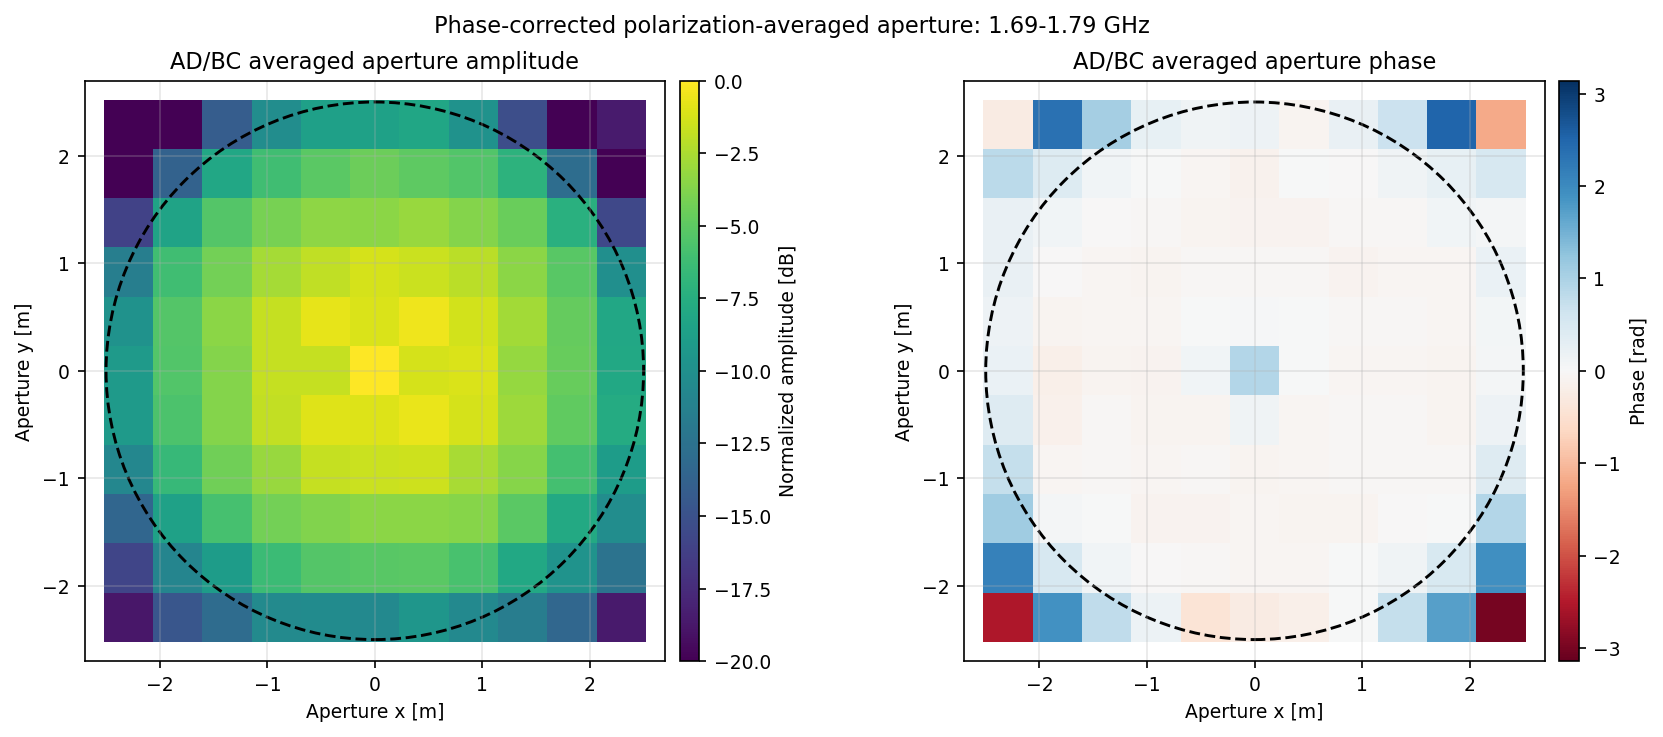
\includegraphics[width=0.95\linewidth]
    {Images/averaged_corrected_aperture.png}
    \caption{Polarization-averaged aperture illumination after independently removing the fitted linear phase gradients from AD and BC. The left panel shows normalized aperture amplitude, and the right panel shows the residual aperture phase.}
    \label{fig:averaged_corrected_aperture}
\end{figure}

The purpose of this correction is specifically to remove the approximately planar phase gradient associated with residual pointing error. Geometric structure outside the physical aperture support is excluded from the analysis and is therefore not relevant to the reconstructed dish surface. Within the physical aperture, the remaining phase structure can contain contributions from the feed illumination pattern (discussed in section \ref{feed}), the non-intersecting antenna axes, residual instrumental effects, and genuine surface errors on the reflector. These terms are not removed by the linear pointing correction and must be interpreted separately when deriving the final surface-error map.


\subsubsection{Phase Map to Surface Error Map}

After reconstructing the complex aperture maps and correcting the residual phase
gradient, the next step is to convert the aperture phase into a physical surface
error map. This is done for each individual cross-correlation aperture and for
the polarization-averaged aperture.

First, a representative wavelength is chosen from the frequency range used to
form the range-averaged aperture. If the mean frequency of the selected channel
range is \(\nu\), then the corresponding wavelength is
Equation~\eqref{eq:wavelength-frequency} gives the wavelength at the observing frequency.
where \(c\) is the speed of light.

For each aperture, the reconstructed complex aperture field
\begin{equation}
A(x,y)
\end{equation}
is converted into a phase map using
\begin{equation}
\phi(x,y) = \arg\!\left[A(x,y)\right].
\end{equation}

This phase is then interpreted as a surface displacement. Because a reflector
surface error produces a round-trip path-length error, the corresponding surface
error is
\begin{equation}
\Delta z(x,y) = \frac{\lambda \phi(x,y)}{4\pi}.
\end{equation}
In millimeters, this is
\begin{equation}
\Delta z_{\rm mm}(x,y)
=
10^3 \frac{\lambda \phi(x,y)}{4\pi}.
\end{equation}

Only the physical dish aperture is retained when computing the surface error.
A circular support mask is applied so that only points satisfying
\begin{equation}
\sqrt{x^2+y^2} \le R_{\rm ap}
\end{equation}
are included, where \(R_{\rm ap}\) is the aperture radius. Points outside the
dish or points with non-finite reconstructed values are excluded.

For each aperture map, the amplitude, phase, and surface error are displayed
together. The aperture amplitude is normalized to its peak and plotted in dB:
\begin{equation}
A_{\rm dB}(x,y)
=
20\log_{10}
\left(
\frac{|A(x,y)|}{\max |A(x,y)|}
\right).
\end{equation}

The phase is shown in degrees,
\begin{equation}
\phi_{\rm deg}(x,y)
=
\frac{180}{\pi}\phi(x,y),
\end{equation}
and the surface error is shown in millimeters using the phase-to-surface
conversion above.

To summarize the surface quality, two scalar metrics are computed inside the
aperture mask. The RMS surface error is
\begin{equation}
\Delta z_{\rm RMS}
=
\sqrt{
\left\langle
\Delta z_{\rm mm}^2
\right\rangle
},
\end{equation}
where the average is taken only over valid points inside the dish aperture. The
peak-to-peak surface error is
\begin{equation}
\Delta z_{\rm P\text{-}P}
=
\max(\Delta z_{\rm mm})
-
\min(\Delta z_{\rm mm}).
\end{equation}
It is also useful to compare the RMS surface error to the wavelength using
\begin{equation}
\frac{\Delta z_{\rm RMS}}{\lambda}.
\end{equation}

In this analysis, the surface maps are generated for the individual
cross-correlation apertures AD and BC, as well as for the polarization-averaged
aperture AD/BC. Comparing these three cases is useful because it shows whether
the inferred surface structure is stable between polarization products and
whether averaging reduces noise while preserving the main large-scale features.

\begin{figure}[H]
    \centering
    \safeincludegraphics[
        width=\linewidth,
        height=0.88\textheight,
        keepaspectratio
    ]{Images/Holography_summary.png}
    \caption{Summary of the reconstructed aperture amplitude, aperture phase, and derived surface error maps for the AD, BC, and polarization-averaged AD/BC apertures. Each row corresponds to one aperture product, while the columns show normalized aperture amplitude in dB, aperture phase in degrees, and surface error in millimeters. The dashed circle marks the physical dish boundary.}
    \label{fig:holography_surface_summary}
\end{figure}

Figure~\ref{fig:holography_surface_summary} provides a compact summary of the
holography result. The first column shows the reconstructed aperture amplitude,
which traces the illumination of the dish. The second column shows the residual
aperture phase after phase-gradient correction. The third column shows the
corresponding surface error map obtained by converting phase into a physical
height error. The similarity between the AD and BC maps, and the cleaner
appearance of the AD/BC average, provide a useful consistency check on the
reconstruction.

\begin{table}[H]
    \centering
    \caption{Surface-error summary for the individual AD and BC aperture reconstructions and the polarization-averaged AD/BC aperture. RMS and peak-to-peak values are computed inside the circular dish aperture mask.}
    \label{tab:surface_error_summary}
    \begin{tabular}{lccc}
        \hline
        Aperture & RMS [mm] & P-P [mm] & RMS/$\lambda$ \\
        \hline
        AD            & 3.90 & 53.88 & 0.0227 \\
        BC            & 3.81 & 58.27 & 0.0221 \\
        AD/BC average & 3.54 & 55.05 & 0.0206 \\
        \hline
    \end{tabular}
\end{table}

Table~\ref{tab:surface_error_summary} shows that the polarization-averaged
AD/BC aperture gives the lowest RMS surface error, \(3.54~\mathrm{mm}\), or
about \(0.0206\lambda\). This suggests that averaging the AD and BC
cross-correlation products reduces noise while preserving the dominant surface
structure.

These surface-error maps are the final physical product of the holography
analysis, since they directly connect the measured beam response to the
mechanical quality of the reflector surface.
\subsection{Making Surface Error Maps 2: Testing Holography Analysis by Introducing Artificial Surface Errors}

\subsubsection{Consideration 4: Phase Pattern from Antenna Feed}\label{feed}
\subsubsection{Consideration 5: Non-intersecting Axes}
\subsection{Making Surface Error Maps 3: Large Holography Maps Integrated Across Multiple Days}
\subsection{Making Surface Error Maps 4: Final Map}

\printbibliography[heading=bibintoc,title={References}] 

\end{document}
